\documentclass[letterpaper,final,12pt,reqno]{amsart}

\usepackage[total={6.3in,9.2in},top=1.1in,left=1.1in]{geometry}

\usepackage{times,bm,bbm,empheq,fancyvrb,graphicx,amsthm,amssymb}
\usepackage[dvipsnames]{xcolor}
\usepackage{longtable}
\usepackage{booktabs}

\usepackage{tabto}
\TabPositions{1.5cm}

\usepackage{tikz}
\usetikzlibrary{decorations.pathreplacing}

\usepackage[kw]{pseudo}
\pseudoset{%
left-margin=15mm,%
topsep=5mm,%
label=\footnotesize\arabic*,%
idfont=\texttt,%
ctfont=\textsl,%
ct-left=\qquad\qquad(,%
ct-right=),%
}

\usepackage{float}

% hyperref should be the last package we load
\usepackage[pdftex,
colorlinks=true,
plainpages=false, % only if colorlinks=true
linkcolor=blue,   % ...
citecolor=Red,    % ...
urlcolor=black    % ...
]{hyperref}

\renewcommand{\baselinestretch}{1.05}

\allowdisplaybreaks[1]  % allow display breaks in align environments, if they avoid major underfulls

\newtheoremstyle{cstyle}% name
  {5pt}% space above
  {5pt}% space below
  {\itshape}% body font
  {}% indent amount
  {\itshape}% theorem head font
  {.}% punctuation after theorem head
  {.5em}% space after theorem head
  {\thmname{#1}\thmnumber{ #2}\thmnote{ (#3)}}% theorem head spec
\theoremstyle{cstyle}

\newtheorem{theorem}{Theorem}
\newtheorem{lemma}[theorem]{Lemma}
\newtheorem{corollary}[theorem]{Corollary}
\newtheorem{assumptions}[theorem]{Assumptions}

\newtheoremstyle{cstyle*}% name
  {5pt}% space above
  {5pt}% space below
  {\itshape}% body font
  {}% indent amount
  {\itshape}% theorem head font
  {.}% punctuation after theorem head
  {.5em}% space after theorem head
  {\thmname{#1}}% theorem head spec
\theoremstyle{cstyle*}
\newtheorem{assumptions*}{Assumptions}

\newtheoremstyle{dstyle}% name
  {5pt}% space above
  {5pt}% space below
  {}%{\itshape}% body font
  {}% indent amount
  {\itshape}% theorem head font
  {.}% punctuation after theorem head
  {.5em}% space after theorem head
  {\thmname{#1}\thmnumber{ #2}\thmnote{ (#3)}}% theorem head spec
\theoremstyle{dstyle}

\newtheorem{definition}[theorem]{Definition}
\newtheorem{example}[theorem]{Example}

% numbering
\numberwithin{equation}{section}
\numberwithin{figure}{section}
\numberwithin{table}{section}
\numberwithin{theorem}{section}

\newcommand{\eps}{\epsilon}
\newcommand{\RR}{\mathbb{R}}

\newcommand{\grad}{\nabla}
\newcommand{\Div}{\nabla\cdot}
\newcommand{\trace}{\operatorname{tr}}

\newcommand{\hbn}{\hat{\mathbf{n}}}

\newcommand{\bb}{\mathbf{b}}
\newcommand{\be}{\mathbf{e}}
\newcommand{\bbf}{\mathbf{f}}
\newcommand{\bg}{\mathbf{g}}
\newcommand{\bn}{\mathbf{n}}
\newcommand{\br}{\mathbf{r}}
\newcommand{\bu}{\mathbf{u}}
\newcommand{\bv}{\mathbf{v}}
\newcommand{\bw}{\mathbf{w}}
\newcommand{\bx}{\mathbf{x}}
\newcommand{\by}{\mathbf{y}}
\newcommand{\bz}{\mathbf{z}}

\newcommand{\bF}{\mathbf{F}}
\newcommand{\bV}{\mathbf{V}}
\newcommand{\bX}{\mathbf{X}}

\newcommand{\bxi}{\bm{\xi}}
\newcommand{\bzero}{\bm{0}}

\newcommand{\cK}{\mathcal{K}}
\newcommand{\cV}{\mathcal{V}}

\newcommand{\rhoi}{\rho_{\text{i}}}

\newcommand{\ip}[2]{\left<#1,#2\right>}

\newcommand{\maxR}{R^{\bm{\oplus}}}
\newcommand{\minR}{R^{\bm{\ominus}}}
\newcommand{\iR}{R^{\bullet}}

\newcommand{\nn}{{\text{n}}}
\newcommand{\pp}{{\text{p}}}
\newcommand{\qq}{{\text{q}}}
\newcommand{\rr}{{\text{r}}}

\newcommand{\supp}{\operatorname{supp}}
\newcommand{\Span}{\operatorname{span}}


\begin{document}
\title[Multilevel constraint decomposition methods]{Multilevel constraint decomposition methods \\ for nonlinear variational inequalities}

\author{Ed Bueler}

\date{\today}

\begin{abstract} FIXME
\end{abstract}

\maketitle

\tableofcontents

\thispagestyle{empty}
%\bigskip

\newfloat{pseudofloat}{t}{xyz}[section]
\floatname{pseudofloat}{Algorithm}


\section{Introduction} \label{sec:intro}

We extend the constraint decomposition (CD) method of X.-C.~Tai \cite{Tai2003} by implementing fully-nonlinear corrections, and we apply it to nonlinear variational inequality (VI) problems to which it has not been applied.  In its multilevel form the method has been shown to have optimal complexity for elliptic, linear obstacle problems \cite[Subsection 5.4]{Tai2003}; see also \cite[Theorem 4.6 and Algorithm 4.7]{GraeserKornhuber2009}.  The convergence of this method, for several types of decompositions, was proven for coercive VI problems which arise from minimization of a convex functional over a convex set \cite{Tai2003}.

The multilevel CD algorithms in \cite{GraeserKornhuber2009} and \cite{Tai2003} are extended here, for finite element (FE) solvers, in three practical ways:
\renewcommand{\labelenumi}{\emph{(\roman{enumi})}}
\begin{enumerate}
\item We apply a full approximation storage (FAS; see \cite{Brandt1977,Bruneetal2015}) approach.  Section \ref{sec:results} shows results from this \emph{nonlinear multilevel constraint decomposition} (NMCD) algorithm  for several nonlinear problems.  Note that this algorithm avoids global (Newton) linearization; compare \cite{GraeserKornhuber2009}.
\item Our implementation permits ``box'' constraints, namely upper and lower obstacles; see Section \ref{sec:femultilevel}.
\item In Sections \ref{sec:femultilevel} and \ref{sec:vcycle} we explain why, given the manner in which constraint sets are decomposed in the multilevel context \cite{GraeserKornhuber2009}, ``up-smoothing'' is more efficient than ``down-smoothing''.  A strong preference for up-smoothing is special to multilevel CD methods and does not arise in unconstrained problems.
\end{enumerate}

The iterates from a CD method are always admissible, and thus the nonlinear operator in the VI need only be defined for admissible states.  Our NMCD scheme is designed for such admissible-only problems, some of which require the solution of an auxiliary PDE on a domain determined inside the VI residual evaluation, as discussed in \cite{Bueler2021conservation}.  NMCD methods should permit direct solutions of those VI problems for which non-admissible methods, including semi-smooth methods \cite{BensonMunson2006}, require unnatural modifications of the operator formula.

One of our examples (Section \ref{sec:results}) demonstrates the application of the NMCD method to a problem of porous-media type, a nonlinear operator which is not known to be coercive.  By ``freezing' the solution-dependent coefficient, the operator is approximated by a coercive operator for the duration of the V-cycle.  This scheme is also effective for doubly-nonlinear diffusion operators.

For the classical obstacle problem with a Laplacian operator, certain multilevel techniques, such as the truncated monotone multigrid method \cite{Kornhuber1994}, are known to improve performance relative to the original multilevel CD method from \cite{Tai2003}; see also \cite{GraeserKornhuber2009}.  These improved methods either track the active set in the discretization or modify the nodal basis functions, and in this sense they are discrete algorithms, while by contrast the CD method applies essentially at the level of the continuum problem; see Section \ref{sec:cd}.  Acceleration of our NMCD method via active-set and/or basis-level manipulations represents a potential extension of the method here, and is a topic for future research.


\section{Coercive variational inequalities} \label{sec:vi}

Suppose $\cV$ is a real and reflexive Banach space with norm $\|\cdot\|$, and denote its topological dual space by $\cV'$.  Denote the dual pairing of $\phi \in \cV'$ and $v\in\cV$ by $\ip{\phi}{v} = \phi(v)$, and note that $\|\phi\|_{\cV'} = \sup_{\|v\|=1} |\ip{\phi}{v}|$ defines a (Banach space) norm on $\cV'$.

Let $\cK \subset \cV$ be a nonempty closed and convex subset, the \emph{constraint set}; elements of $\cK$ are said to be \emph{admissible}.  For a continuous, but generally nonlinear, operator $f:\cK \to \cV'$ and a linear \emph{source functional} $\ell\in \cV'$ we consider the following \emph{variational inequality} (VI) problem for the (exact) solution $u^*\in \cK$, if it exists:
\begin{equation}
\ip{f(u^*)}{v-u^*} \ge \ip{\ell}{v-u^*} \qquad \text{for all } v\in \cK. \label{eq:vi}
\end{equation}
Because $f$ is (generally) nonlinear, the source term $\ell$ is not strictly needed, and indeed by redefining $f$ we may take $\ell=0$, but its presence clarifies the algorithm in Section \ref{sec:vcycle}.

VI \eqref{eq:vi} generalizes the nonlinear system of equations $f(u^*)=\ell$ to problems where $u^*$ is also required to be in a constraint set $\cK$.  Informally, if we conceptualize the dual pairing as an inner product, then \eqref{eq:vi} says that the angle between $f(u^*)-\ell$ and any arbitrary vector $v-u$ pointing from $u$ into $\cK$ is at most $90^\circ$.  That is, while $f(u^*)-\ell$ may not be zero, it must point directly into $\cK$.  On the other hand, if $u^*$ is in the interior of the constraint set, i.e.~$u^*\in\cK^\circ$, then \eqref{eq:vi} implies $f(u^*)=\ell$.

\begin{definition} The following definitions are standard \cite{KinderlehrerStampacchia1980}.  A map $f:\cK \to \cV'$ is \emph{monotone} if
\begin{equation}
\ip{f(u)-f(v)}{u-v} \ge 0 \qquad \text{for all } u,v \in \cK, \label{eq:monotone}
\end{equation}
\emph{strictly monotone} if equality in \eqref{eq:monotone} implies $u=v$, and \emph{coercive} if there exists $w \in \cK$ so that
\begin{equation}
\frac{\ip{f(u)-f(w)}{u-w}}{\|u-w\|} \to +\infty \qquad \text{as } \|u\|\to +\infty. \label{eq:coercive}
\end{equation}
\end{definition}

It is well-known that if $f:\cK \to \cV'$ is continuous, monotone, and coercive then VI \eqref{eq:vi} has a solution \cite[Corollary III.1.8]{KinderlehrerStampacchia1980}, and that the solution is unique when $f$ is strictly monotone.  As in the calculus of variations \cite{Evans2010}, coercivity permits a compactness argument for unbounded sets $\cK$.  (Recall that the closed and bounded subsets of a reflexive Banach space are weakly compact.)  The condition of continuity can be weakened, e.g.~to only apply on finite-dimensional subspaces \cite{KinderlehrerStampacchia1980}, but the stronger condition will apply in our examples.

The coercive VIs solved in this paper satisfy a stronger inequality than \eqref{eq:coercive}.

\begin{definition}  Let $p>1$.  The map $f:\cK \to \cV'$ is \emph{$p$-coercive} if there exists $\kappa>0$ such that
\begin{equation}
\ip{f(u)-f(v)}{u-v} \ge \kappa \|u-v\|^p \qquad \text{for all } u,v \in \cK. \label{eq:pcoercive}
\end{equation}
\end{definition}

It is easy to see that if $f$ is $p$-coercive then it is monotone, strictly monotone, and coercive, so the following well-posedness theorem holds.

\begin{theorem}  \label{thm:viwellposed}  If $f:\cK \to \cV'$ is continuous and $p$-coercive then there exists a unique $u^*\in \cK$ solving VI \eqref{eq:vi}.
\end{theorem}

When $f$ is monotone, VI \eqref{eq:vi} generalizes the problem of minimizing a convex function over $\cK$.  In fact, suppose $F:\cK \to \RR$ is lower semi-continuous and (G\^ateau) differentiable with continuous derivative $F':\cK \to \cV'$.  Then $F$ is convex if and only if $F'$ is monotone \cite[Proposition I.5.5]{EkelandTemam1976}.  Furthermore, Proposition II.2.1 in \cite{EkelandTemam1976} shows that if $F$ is convex then \eqref{eq:vi} holds for $f=F'$ if and only if
\begin{equation}
u^* = \operatorname{arg-min}_{v\in\cK} F(v) - \ip{\ell}{v}. \label{eq:minimization}
\end{equation}
The CD methods of Tai \cite{Tai2003} address problem \eqref{eq:minimization} under the hypotheses that such an objective $F$ exists, and that $F'$ is 2-coercive.  (Note that Tai \cite{Tai2003} uses ``coercive'' for what we call $2$-coercive.)

The problems addressed later in Section \ref{sec:results} involve nonlinear and linear operators $f$ which are partial differential operators.  As described in section \ref{sec:femultilevel}, the constraint sets $\mathcal{K}$ incorporate both inequality box constraints and nonhomogeneous Dirichlet boundary conditions as equality constraints.  However, the following examples use homogeneous (zero) Dirichlet conditions for ease of presentation.

Let $\Omega \subset \RR^d$ denote a bounded, open set with smooth or piecewise-smooth (e.g.~polygonal) boundary.  Sobolev spaces \cite{Evans2010} are denoted by $W^{k,p}(\Omega)$, for integer $k$ and $1\le p \le \infty$.  The following example includes the classical obstacle problem for the linear Laplacian \cite{GraeserKornhuber2009} and the $p$-Laplacian for $p\ge 2$ \cite{ChoeLewis1991}.

\begin{example}  \label{ex:plaplacian}  Suppose $a\in L^\infty(\Omega)$ such that $a(x)\ge a_0$ a.e.~for some constant $a_0>0$, and $p\ge 2$.  For $u,v \in \cV = W^{1,p}_0(\Omega)$ define $f:\cV \to \cV'$ by
\begin{equation}
\ip{f(u)}{v} = \int_\Omega a(x) |\grad u|^{p-2} \grad u \cdot \grad v\,dx, \label{eq:plaplacian}
\end{equation}
a continuous map \cite[Theorem A.0.6]{Peral1997}.  Now, if $x,y\in\RR^d$ then $(|x|^{p-2} x - |y|^{p-2} y)\cdot (x-y) \ge 2^{2-p} |x-y|^p$ \cite[see Appendix A and references therein]{Bueler2021conservation}.  Thus it follows from the Poincar\'e inequality that
    $$\ip{f(u) - f(v)}{u-v} \ge 2^{2-p} a_0 \|\grad u - \grad v\|_p^p \ge 2^{2-p} a_0 C \|u-v\|^p$$
for some $C>0$, and thus $f$ is $p$-coercive.  On the other hand, for $\ell\in\cV'$ define
    $$F(v) = \int_\Omega \frac{a(x)}{p} |\grad v|^p\,dx - \ip{\ell}{v}.$$
Then $F$ is a convex functional and $F'(v) = f(v) - \ell$ for $f$ given in \eqref{eq:plaplacian}.  For any closed and convex $\cK\subset \cV$, VI problem \eqref{eq:vi} for $f$ is equivalent to optimization problem \eqref{eq:minimization} for $F$.\end{example}

The map in \eqref{eq:plaplacian} is also coercive if $1<p<2$, but the proof is somewhat different \cite[Theorem 4.4]{Bueler2021conservation}.  In Section \ref{sec:results} we consider only the $p\ge 2$ case.

However, not all VI problems arise from optimization.  We give two such examples next, first a coercive and linear advection-diffusion problem, and then a nonlinear porous-medium-type problem.  The first is preceded by a lemma.

\begin{lemma}  \label{lem:advectionskew}  \cite{Elmanetal2014}\,  Suppose $\bX :\Omega \to \RR^d$ is a bounded and boundedly-differentiable vector field on $\Omega$ with zero divergence ($\Div \bX=0$).  For $u,v \in W^{1,2}(\Omega)$ let $b(u,v) = \int_\Omega (\bX \cdot \grad u) v\,dx$.  Then $b(u,u) = \frac{1}{2} \int_{\partial \Omega} u^2 \bX\cdot \bn\,dx$ where $\bn$ is the outward normal on $\partial \Omega$.
\end{lemma}

\begin{proof}
Integration by parts gives $b(u,v) = - b(v,u) + \int_{\partial \Omega} uv \bX\cdot \bn\,dx$, so the result follows.
\end{proof}

\begin{example}  \label{ex:advectiondiffusion}  Suppose $\partial\Omega$ is partitioned into Dirichlet and Neumann portions, i.e.~$\partial\Omega = \partial_D\Omega \cup \partial_N\Omega$, with $\partial_D\Omega$ of positive measure.  Let $\cV = W_0^{1,2}(\Omega)$ be the space of functions which are zero along $\partial_D\Omega$.  Consider a divergence-free velocity field $\bX$ on $\Omega$ satisfying the conditions of Lemma \ref{lem:advectionskew}, but additionally assume that the flow is outward on the Neumann boundary, $\bX \cdot \bn \ge 0$ on $\partial_N\Omega$.  For $u,v \in \cV = W_0^{1,2}(\Omega)$ and $\eps>0$ define
\begin{equation}
\ip{f(u)}{v} = \eps \left(\grad u, \grad v\right)_{L^2(\Omega)} - b(u,v). \label{eq:advectiondiffusion}
\end{equation}
Consider VI \eqref{eq:vi} for any closed and convex $\cK \subset \cV$ and $g\in\cV'$.  It is easy to see that $|\ip{f(u)}{v}| \le (\eps + \|\bX\|_\infty) \|u\| \|v\|$, thus that $f:\cK \to \cV'$ is continuous.  Lemma \ref{lem:advectionskew} says that the bilinear form $s(u,v)$ is skew-symmetric up to a nonnegative term.  By the outward flow assumption and the Poincar\'e inequality,
\begin{align*}
\ip{f(u)-f(v)}{u-v} &= \eps \int_\Omega |\grad u - \grad v|^2\,dx + b(u-v,u-v) \\
                    &= \eps \int_\Omega |\grad u - \grad v|^2\,dx + \frac{1}{2} \int_{\partial_N\Omega} (u-v)^2 \bX\cdot\bn \ge \eps C \|u-v\|^2.
\end{align*}
Thus $f$ is 2-coercive, and so VI problem \eqref{eq:vi} is well-posed.
\end{example}

References \cite{Bueler2021conservation,ChangNakshatrala2017} consider advection-diffusion VI problems like Example \ref{ex:advectiondiffusion}, specifically over the set $\cK = \{v\ge 0\}$.  If $\bX \ne 0$ then VI \eqref{eq:vi} for $f$ in \eqref{eq:advectiondiffusion} does not correspond to a minimization problem.  Indeed, $\ip{f(u)}{v}$ is not symmetric in that case, so $f$ cannot be the gradient of a scalar objective.  To see this, assume $\bX \ne 0$ is continuous for simplicity.  For $u,v$ which are zero on $\partial \Omega$, note $\ip{f(u)}{v} - \ip{f(v)}{u} = -2 b(u,v)$.  By constructing $u,v$ locally near some point where $\bX$ is nonzero one may show $b(u,v)\ne 0$.

\begin{example}  \label{ex:porous}  Suppose $\phi:[0,\infty) \to [\phi_0,\infty)$ is continuous for some constant $\phi_0>0$.  Then the following operator, of porous medium type, is not known to be monotone (or coercive) when $\phi$ is not constant:
\begin{equation}
\ip{f(u)}{v} = \int_\Omega \phi(u) \grad u \cdot \grad v\,dx. \label{eq:porous}
\end{equation}
As with Example \ref{ex:advectiondiffusion}, this form does not have the symmetry necessary to be the gradient of a scalar objective.
\end{example}

Numerical solver performance for Examples \ref{ex:plaplacian}, \ref{ex:advectiondiffusion}, and \ref{ex:porous} will be considered in Section \ref{sec:results}.  Further examples of nonlinear VI problems appear in ice sheet models \cite{Calvoetal2002,JouvetBueler2012} and other geophysical fluids.


\section{Constraint decomposition (CD)} \label{sec:cd}

Suppose there are $m<\infty$ closed subspaces $\cV_i \subset \cV$ so that the sum
\begin{equation}
\cV = \sum_{i=0}^{m-1} \cV_i \label{eq:subspacedecomp}
\end{equation}
holds in the sense that if $w \in \cV$ then there exist $w_i \in \cV_i$ so that $w = \sum_i w_i$.  Equation \eqref{eq:subspacedecomp} is called a \emph{subspace decomposition} of $\cV$ \cite{Xu1992}.

Suppose further that $\cK_i \subset \cV_i$ are nonempty, closed, and convex subsets such that
\begin{equation}
\cK = \sum_{i=0}^{m-1} \cK_i \label{eq:constraintdecomp}
\end{equation}
for a closed, convex subset $\cK \subset \cV$, as considered in the previous section.  The sum in \eqref{eq:constraintdecomp} is required to hold in two senses \cite{TaiTseng2002}: \emph{(i)}~if $w \in \cK$ then there exist $w_i \in \cK_i$ so that $w = \sum_i w_i$, and \emph{(ii)}~if $z_i \in \cK_i$ for each $i$ then $\sum_i z_i \in \cK$.  Observe that sense \emph{(ii)} is automatic for \eqref{eq:subspacedecomp} because the $\cV_i$ are subspaces.  Note that neither decomposition \eqref{eq:subspacedecomp} or \eqref{eq:constraintdecomp} is required to be unique.  Also, $\cK_i \not\subset \cK$ in many applications; see the cartoon in Figure \ref{fig:cartoon}.

Finally, for each $\cK_i$ suppose there are bounded, generally-nonlinear \emph{decomposition operators}\footnote{Denoted ``$R_i$'' in \cite{Tai2003}.  Here we avoid a notational conflict with multilevel transfer operators (Section \ref{sec:femultilevel}).} $\Pi_i : \cK \to \cK_i$ such that if $v \in \cK$ then
\begin{equation}
v = \sum_{i=0}^{m-1} \Pi_i v.  \label{eq:constraintrestrictionsum}
\end{equation}
Clearly \eqref{eq:constraintrestrictionsum} implies sense \emph{(i)} for \eqref{eq:constraintdecomp}. A \emph{constraint decomposition} (CD) of $\cK$ is a choice of $\cV_i,\cK_i,\Pi_i$ satisfying \eqref{eq:subspacedecomp}--\eqref{eq:constraintrestrictionsum} \cite{Tai2003}.  Figure \ref{fig:cartoon} suggests how a low-dimensional example might look.

\begin{figure}[ht]
\includegraphics[width=0.6\textwidth]{genfigs/cartoon.pdf}
\caption{Suppose $\mathcal{V}$ is the space of real functions on a two-point set $\Omega=\{x_1,x_2\}$.  A constraint decomposition (CD) for a unilateral obstacle problem with $\mathcal{K}=\{v\ge \psi\}$ might look like this.}
\label{fig:cartoon}
\end{figure}

In Sections \ref{sec:femultilevel} and \ref{sec:vcycle} we will introduce discretizations and practical algorithms for finite-dimensional VI problems.  However, one can observe that the CD concept applies at the level of the continuum problem, and the following two obstacle problem examples are illustrations.  The first is an overlapping domain decomposition.

\begin{example}  \label{ex:domaindecomposition}  For a bounded domain $\Omega \subset \RR^d$, let $\cV = W_0^{k,p}(\Omega)$ for $k\ge 0$ and $p\ge 1$.  Suppose an obstacle $\psi \in W^{k,p}(\Omega)$ satisfies $\psi|_{\partial \Omega} \le 0$, and let $\cK = \{v \ge \psi\} \subset \cV$.  Suppose further that $\{\phi_i\}_{i=0}^{m-1}$ is a smooth partition of unity on $\Omega$, satisfying $0 \le \phi_i\le 1$ and $\sum_i \phi_i = 1$, and let $\Omega_i$ be the open support of $\phi_i$.  Let $\cV_i = \{w \in \cV:w|_{\Omega \setminus \Omega_i} =0 \}$, $\cK_i = \{v \in \cV_i: v \ge \phi_i \psi\}$, and $\Pi_i(v) = \phi_i v$.  Then \eqref{eq:subspacedecomp}, \eqref{eq:constraintdecomp}, and \eqref{eq:constraintrestrictionsum} all hold.
\end{example}

Our second example is a disjoint frequency decomposition.  A multilevel CD over a finite-dimensional FE discretization, specifically the one proposed in Section \ref{sec:femultilevel}, approximates such a frequency decomposition.

\begin{example}  \label{ex:frequencydecomposition}  For simplicity suppose $\Omega = (0,a)^d \subset \RR^d$ is a cube, and let $\cV = W_{\text{per}}^{p,k}(\Omega)$, for $p\ge 2$ and $k\ge 0$, be the periodic functions.  Suppose $\psi \in W_{\text{per}}^{p,k}(\Omega)$ and let $\cK = \{v \ge \psi\} \subset \cV$.  Without using any detailed notation for Fourier representation, but noting that the frequencies are discrete because $\Omega$ is compact, suppose $\{\cV_i\}$ are $m<\infty$ subspaces of $\cV$ defined by an (nonoverlapping) partition of $W_{\text{per}}^{p,k}(\Omega)$ by frequency, thus satisfying \eqref{eq:subspacedecomp} as an orthogonal decomposition.  Suppose $P_i:\cV \to \cV_i$ are the corresponding orthogonal projections, satisfying $I = \sum_i P_i$.  Let $\cK_i = \{v \ge P_i \psi\} \subset \cV_i$ and $\Pi_i = P_i$.  Then \eqref{eq:constraintdecomp} and \eqref{eq:constraintrestrictionsum} also hold.
\end{example}

Again note that $\cK_i \not\subset \cK$ in these cases.\footnote{Informally speaking, the important inclusion is $\cK_i \subset \cV_i$.}  In Example \ref{ex:domaindecomposition}, if $\psi$ is positive over portions of $\Omega$ where the decomposition into overlapping subdomains $\Omega_i$ is nontrivial, then $\cK_i \not\subset \cK$, and something similar holds for Example \ref{ex:frequencydecomposition}.


\section{Basic CD iterations} \label{sec:cditers}

Associated to a constraint decomposition (CD) are certain basic iterative methods.  Algorithms \ref{alg:basiccd-add} and \ref{alg:basiccd-mult} below are functions which improve a current iterate $u \in \cK$, generating output $w\in\cK$ which should be closer to the solution $u^* \in \cK$ of \eqref{eq:vi}, by solving smaller VI problems over each CD subset $\cK_i$.   The two Algorithms each permit a damping parameter $0<\alpha\le 1$, and they generalize the Jacobi and Gauss-Seidel iterations, respectively.

In Algorithm \ref{alg:basiccd-add}, the additive or parallel CD method, ``\textbf{for all}'' can be computed in any order.  Note that the expression ``$u-\Pi_iu+\hat w_i$'' removes the part of $u$ which lies in $\mathcal{K}_i$ before adding-back the improved subset solution $\hat w_i \in \mathcal{K}_i$.

\begin{pseudofloat}[H]
\begin{pseudo*}
\pr{cd-add}(u)\text{:} \\+
    for all $i \in \{0,\dots,m-1\}$: \\+
        \rm{find} $\hat w_i\in \cK_i$ \rm{so that for all} $v_i\in \cK_i$, \\+
            $\boxed{\ip{f(u - \Pi_i u + \hat w_i)}{v_i-\hat w_i} \ge \ip{\ell}{v_i-\hat w_i}}$ \\--
    $\hat w = \sum_i \hat w_i\in\cK$ \\
    return $w=(1-\alpha) u + \alpha \hat w$
\end{pseudo*}
\caption{One additive CD iteration for VI problem \eqref{eq:vi}.}
\label{alg:basiccd-add}
\end{pseudofloat}

In the multiplicative (successive) version, Algorithm \ref{alg:basiccd-mult}, each $\mathcal{K}_i$ solution corrects the global iterate immediately, and the $\mathcal{K}_i$ are addressed in a fixed order.  The sum ``$\sum_{j>i} \Pi_j u$'' should be read as keeping the parts of the input $u$ which have not yet improved.   Note we must update the subset iterate $w_i$ using the same damping that is applied to the final output $w$.

\begin{pseudofloat}
\begin{pseudo*}
\pr{cd-mult}(u)\text{:} \\+
    for $i = 0,\dots,m-1$: \\+
        \rm{find} $\hat w_i\in \cK_i$ \rm{so that for all} $v_i\in \cK_i$, \\+
            $\displaystyle \boxed{\ip{f\Big(\sum_{j<i} w_j + \hat w_i + \sum_{j>i} \Pi_j u\Big)}{v_i-\hat w_i} \ge \ip{\ell}{v_i-\hat w_i}}$ \\-
            $w_i = (1-\alpha) \Pi_i u + \alpha \hat w_i\in\cK_i$ \\-
    $\hat w = \sum_i \hat w_i\in\cK$ \\
    return $w=(1-\alpha) u + \alpha \hat w$
\end{pseudo*}
\caption{One multiplicative CD iteration for VI problem \eqref{eq:vi}.}
\label{alg:basiccd-mult}
\end{pseudofloat}

In each boxed VI the argument of $f$ is an element of $\cK$, as the reader should confirm.  On the other hand, by \eqref{eq:constraintdecomp} and \eqref{eq:constraintrestrictionsum} one may also write the test vector $v_i - \hat w_i \in \cV_i$ as a difference of admissible vectors from $\cK$.  For the two Algorithms respectively:
\begin{align*}
[u - \Pi_i u + v_i] - [u - \Pi_i u + \hat w_i] &= v_i - \hat w_i, \label{eq:admissibledifference} \\
\left[\sum_{j<i} w_j + v_i + \sum_{j>i} \Pi_j u\right] - \left[\sum_{j<i} w_j + \hat w_i + \sum_{j>i} \Pi_j u\right] &= v_i - \hat w_i.  \notag
\end{align*}
In this sense the boxed VIs are for the same problem as the original VI \eqref{eq:vi}.

For either Algorithm we define the $i$th \emph{subset update} as
\begin{equation}
e_i = \hat w_i - \Pi_i u \in \cV_i. \label{eq:ithupdate}
\end{equation}
The reader may check that $\hat w = u + \sum_{i} e_i$ and $w = u + \alpha \sum_i e_i$.  Trivially, $\hat w = u^* + \sum_i \hat w_i - \Pi_i u^*$ also holds.

We will refer to Algorithms \ref{alg:basiccd-add} and \ref{alg:basiccd-mult} as the \emph{basic CD iterations}.  These iterations are meaningful even when $f$ is nonlinear, non-local, or defined only on $\cK$.  However, practical and efficient FE implementation for such general operators $f$ seems not to have been addressed in the literature, and doing so will require new notions.  In particular, references \cite{GraeserKornhuber2009,Tai2003} only apply the CD method to the classical obstacle problem for which $f$ is linear, local, and defined for all inputs (i.e.~$f$ is defined on all of $\mathcal{V}$).  The following example exposes the implementation simplifications available in that easier case.

\begin{example}  \label{ex:fnice} Suppose $f:\cV \to \cV'$ is linear.  Furthermore suppose $f$ is a differential operator, thus local in the sense that for any $z\in\mathcal{V}$ the value $\ip{f(\phi)}{z}$ can be computed by an integral over the support of $\phi \in \mathcal{V}$.  Considering additive Algorithm \ref{alg:basiccd-add} for concreteness, by linearity the boxed VI can be written as
\begin{equation}
\ip{f(e_i)}{v_i-\hat w_i} \ge \ip{\tilde\ell}{v_i-\hat w_i}, \label{eq:linearlocalvi}
\end{equation}
for all $v_i \in \mathcal{K}_i$, where $\tilde\ell = \ell - f(u)$.  Note $e_i = \hat w_i - \Pi_i u \in \cV_i$ is not generally admissible ($e_i \notin \cK$), but \eqref{eq:linearlocalvi} makes sense because $f$ is defined over $\cV$.  Each problem \eqref{eq:linearlocalvi} can be solved using a stored residual $f(u)$, now included into $\tilde\ell$.  If a hat function basis exists for $\cV_i$, namely a basis of small-support functions, then by linearity of $f$ a solver for VI \eqref{eq:linearlocalvi} can be implemented using only integrals over the hat function supports.\footnote{Compare equations (2.31) and (2.32) in \cite{Farrelletal2021}, which describe the same sense of locality.}
\end{example}

When $f$ has all the nice properties listed in Example \ref{ex:fnice} then a solver can take advantage of implementation efficiencies which are unavailable in general.  An FE approximation of VI \eqref{eq:vi}---see Sections \ref{sec:femultilevel} and \ref{sec:vcycle}---can then be solved in any incremental and efficient manner following the techniques in \cite{GraeserKornhuber2009,Tai2003}, namely by computations over hat function supports.  The actual solution process for VI \eqref{eq:linearlocalvi} is not really the concern here; we are observing that the storage needed for problem \eqref{eq:linearlocalvi}, and the cost of residual evaluation, are substantially smaller than in the general case.

For general problems lacking the niceties of Example \ref{ex:fnice}, certain additional ideas are needed for practical implementation.  Section \ref{sec:vcycle} constructs a multilevel CD iteration for functions $f:\cK\to\cV'$, i.e.~defined only on the constraint set, and assuming neither linearity nor locality, by applying the full approximation storage (FAS) idea of Brandt \cite{Brandt1977}.

Specifically for a non-local integral operator $f$, the expression $\ip{f(\phi)}{z}$ requires an integral over $\Omega$ even if $\phi$ is a function with small support (such as a hat function); cf.~subsection 4.5 in \cite{Bueler2021conservation}.  While Algorithm \ref{alg:nmcd} applies, as stated, to such $f$, practical extension of multilevel CD methods to non-local operators is a topic for future research.


\section{Multilevel finite elements} \label{sec:femultilevel}

From now on we are concerned with the approximate solution of certain nonlinear VI problems over 2D computational domains.  Suppose $\Omega \subset \RR^2$ is a (open) bounded polygon and that $\mathcal{V}=W^{1,p}(\Omega)$ is a Sobolev space of once-differentiable functions.  Though the free boundaries are defined by inequality constraints (below), fixed boundary conditions may be Dirichlet or mixed.  Suppose that the domain boundary is split into disjoint, measurable sets, $\partial\Omega = \partial_D \Omega \cup \partial_N \Omega$, with $\partial_D \Omega$ of positive measure for simplicity, to permit well-posedness \cite{Evans2010}, and $\partial_N \Omega$ possibly empty.  Suppose that the provided Dirichlet data $g_D:\partial_D \Omega \to \RR$ is sufficiently-regular to permit well-posedness of the VI problem stated below.

We restrict to the case of \emph{box constraints} \cite{BensonMunson2006,FerrisPang1997}, equivalently \emph{bi-obstacle problems}.  The \emph{lower obstacle} $\underline{\gamma}$ and the \emph{upper obstacle} $\overline{\gamma}$ are given measurable functions on $\overline{\Omega}$ which take their values in the extended real line $\tilde\RR = [-\infty,+\infty]$.  Specifically suppose $\underline{\gamma} : \overline{\Omega} \to [-\infty,+\infty)$ and $\overline{\gamma} : \overline{\Omega} \to (-\infty,+\infty]$ are measurable, satisfying $\underline{\gamma} \le \overline{\gamma}$ on $\overline{\Omega}$ and $\underline{\gamma} \le g_D \le \overline{\gamma}$ on $\partial_D \Omega$.

Now define the constraint set
\begin{equation}
\cK = \left\{w\,:\,\underline{\gamma} \le w \le \overline{\gamma} \,\text{ over }\, \Omega, \, \text{ and }\, w\big|_{\partial_D \Omega} = g_D\right\} \subset \cV =W^{1,p}(\Omega).
\end{equation}
(The boundary values are, as usual, in the trace sense \cite{Evans2010}.)  It is easy to check that $\cK$ is closed and convex.  This definition of $\cK$ treats the inequality and equality (boundary) constraints in a unified manner.

We will solve the same VI as in abstract problem \eqref{eq:vi}.  Given continuous $f:\cK \to \cV'$, and $\ell \in \cV'$, we assume that the following VI is well-posed for $u^*\in \cK$:
\begin{equation}
\ip{f(u^*)}{v-u^*} \ge \ip{\ell}{v-u^*} \qquad \text{for all } v\in \cK. \label{eq:boxdirichletvi}
\end{equation}
Note that $v-u^* \in W_0^{1,p}(\Omega)$, that is, the test functions used in \eqref{eq:boxdirichletvi} have zero values on the Dirichlet boundary $\partial_D\Omega$.

Problem \eqref{eq:boxdirichletvi} is both a free-boundary problem, because of the inequality constraints in defining $\cK$, and a (mixed) fixed-boundary value problem.   Dirichlet conditions $u=g_D$ apply over $\partial_D\Omega$ and Neumann conditions over $\partial_N \Omega$.  The latter are determined by the formula for $f$; for nonhomogeneous Neumann conditions, the nonlinear operator $f:\cK\to\cV'$ will include an integration over $\partial_N\Omega$.

We now construct a multilevel finite element (FE) approximation to problem \eqref{eq:boxdirichletvi} using either triangular or quadrilateral meshes over $\Omega$, and $P_1$ or $Q_1$ elements \cite{Elmanetal2014}, respectively.  The solution on the finest-level mesh, in a hierarchy of meshes constructed by refinement of a coarsest mesh, is the target.   This hierarchy also generates a multilevel CD of $\cK$.  The subsets $\cK_i$ in this CD are designed to allow multigrid-type coarser-level corrections (next Section) in a manner which preserves admissibility, while not introducing unnecessary high frequencies into the coarser-level problems, especially at the free boundary.

The mesh hierarchy and FE spaces are constructed by nested refinement in the following standard manner \cite{Elmanetal2014}.  Suppose $\mathcal{T}^0$ is the \emph{coarsest mesh}, a finite set of non-overlapping, nondegenerate elements (triangles or quadrilaterals) with union equal to $\overline{\Omega}$ and maximum edge length (characteristic size) $h_0>0$.  For $j=1,\dots,J$, let $\mathcal{T}^j$ be the uniform refinement of $\mathcal{T}^{j-1}$ by connecting the midpoints of edges.  For triangles and rectangles, each $\mathcal{T}^{j-1}$ element becomes four similar elements in $\mathcal{T}^j$ with size $h_j = 2^{-j} h_0$.\footnote{For arbitrary triangles, and for rectangles, the refinement generates similar elements and $h_j=2^{-j}h_0$ is the exact maximum edge length in $\mathcal{T}^j$.  For general quadrilaterals, however, similarity is lost and maximum edge lengths are variable; cf.~\cite{Zhang2004}.  Only rectangular quadrilaterals are used in the Results section.}  We call $J\ge 0$ the \emph{depth} of the hierarchy and $\mathcal{T}^J$ the \emph{finest mesh}.  Let $m_j$ be the number of nodes in $\mathcal{T}^j$, the \emph{degrees of freedom} at the $j$th level, and denote $h=h_J=2^{-J} h_0$ and $m=m_J$ for the finest level.  Let $\mathcal{V}^j$ be the continuous $P_1$ or $Q_1$ FE space \cite{Elmanetal2014} over $\mathcal{T}^j$, with arbitrary boundary values, and observe the following vector space nesting:
\begin{equation}
\mathcal{V}^0 \subset \mathcal{V}^1 \subset \dots \subset \mathcal{V}^J \subset \mathcal{V}=W^{1,p}(\Omega).  \label{eq:fe:nestedspaces}
\end{equation}

Use of higher-order Lagrange elements $P_k$ or $Q_k$, $k\ge 2$, would be a ``variational crime'' \cite[Chapter 10]{BrennerScott2007}, specific to inequality constraints, in the upcoming material.  For this reason we restrict to $k = 1$.  Specifically, our FE construction of constraint sets will require \emph{nodal monotonicity}, namely that for all FE functions $w,z \in \mathcal{V}^j$,
\begin{equation}
\bw \ge \bz \quad \implies \quad w \ge z \label{eq:nodalmonotonicity}
\end{equation}
where $\bw,\bz$ denote vectors of nodal values.  For $k\ge 2$ there are hat functions in $P_k$ and $Q_k$, i.e.~functions with nodal value one at a single node, otherwise zero, which take on negative values \cite[Figure 1.7]{Elmanetal2014}.  It is easy to show that \eqref{eq:nodalmonotonicity} is equivalent to the non-existence of sign-changing hat functions, so \eqref{eq:nodalmonotonicity} implies $k\le 1$.

To accomodate the fixed-boundary conditions, let $g_D^J \in \mathcal{V}^J$, on the finest-level mesh, satisfy $g_D^J = g_D$ on $\partial_D \Omega$.\footnote{As is standard in conforming FE methods, this restricts the original Dirichlet boundary values $g_D$ to be a piecewise-linear function \cite{Elmanetal2014}.}  To allow box constraints, let $\tilde{\mathcal{V}}^j$ denote the set of all functions on the nodes of $\mathcal{T}^j$ with values in the extended real line $\tilde{\RR} = [-\infty,+\infty]$.  (Note that $\tilde{\mathcal{V}}^j$ functions are not in $\mathcal{V}^j$.  They are not even defined everywhere on $\Omega$, but only on nodes.)  Suppose that the \emph{lower} and \emph{upper obstacles} $\underline{\gamma}^J, \overline{\gamma}^J \in \tilde{\mathcal{V}}^J$, defined on the nodes of the finest-level mesh $\mathcal{T}^J$, satisfy
\begin{equation}
\underline{\gamma}^J \le \overline{\gamma}^J, \qquad \underline{\gamma}^J < +\infty, \qquad -\infty < \overline{\gamma}^J. \label{eq:fe:boxconstraintrequirements}
\end{equation}
Where $\underline{\gamma}^J=-\infty$ or $\overline{\gamma}^J=+\infty$ then there is no lower or upper constraint, respectively.  Finally assume that $\underline{\gamma}^J \le g_D^J \le \overline{\gamma}^J$ on nodes of $\mathcal{T}^J$ which lie in $\partial_D \Omega$.

Define
\begin{equation}
\mathcal{K}^J = \left\{w\,:\,\underline{\gamma}^J \le w \le \overline{\gamma}^J, \, \text{ and } \, w|_{\partial_D\Omega} = g_D|_{\partial_D\Omega}\right\} \subset \mathcal{V}^J, \label{eq:fe:fineconstraintset}
\end{equation}
as the finest-level \emph{constraint set} of \emph{admissible} FE functions.  This is a nonempty, closed, and convex subset of $\mathcal{V}^J$.  As $\mathcal{V}^J$ functions never take values $\pm\infty$, inequality in \eqref{eq:fe:fineconstraintset} is strict where $\underline{\gamma}^J, \overline{\gamma}^J = \pm \infty$.

Let $f^J:\mathcal{K}^J \to (\mathcal{V}^J)'$ be a discretization of $f$ in \eqref{eq:boxdirichletvi}.  By inclusion \eqref{eq:fe:nestedspaces} the functional $\ell$ is already defined and continuous over $\mathcal{V}^J$, but we denote $\ell^J \in (\mathcal{V}^J)'$ for its FE representation.  We seek the FE solution $u^J \in \mathcal{K}^J$ of the finest-level, finite-dimensional, nonlinear VI
\begin{equation}
\ip{f^J(u^J)}{v-u^J} \ge \ip{\ell^J}{v-u^J} \qquad \text{for all } v\in \cK^J. \label{eq:fe:vi}
\end{equation}
As is true for \eqref{eq:vi}, if $f^J$ is continuous and $p$-coercive on $\mathcal{K}^J$, in the sense that \eqref{eq:pcoercive} holds for all $u,v \in \mathcal{K}^J$, then \eqref{eq:fe:vi} is well-posed.

While \eqref{eq:fe:vi} approximates \eqref{eq:boxdirichletvi}, it may not technically be conforming for that VI.  That is, even if quadrature and other implementation details for $f^J$ are ignored, and despite the vector space inclusion $\mathcal{V}^J \subset \mathcal{V}$, we still do not require $\mathcal{K}^J \subset \mathcal{K}$.  The continuum constraint set $\mathcal{K}$ remains abstract in those applications where only the nodal obstacles $\underline{\gamma}^J, \overline{\gamma}^J$ are defined.  In fact, even if smooth continuum obstacles exist, admissibility with respect to their FE interpolants will generally not imply continuum admissiblity.\footnote{Such caveats apply in geophysical situations where the obstacle is given by meshed elevation data, the continuum limit of which is generally unknown \cite{Bueler2016}.}

Finite-dimensional, box-constrained VI problem \eqref{eq:fe:vi} is equivalent to a \emph{mixed complementarity problem} (MCP) \cite{FacchineiPang2003,FerrisPang1997}.  Stating this strong-form problem may be clarifying for some readers.  Denoting $x_p$ for nodes of the finest-level mesh $\mathcal{T}^J$, let $X=\big\{w\in\cV^J\,:\,w(x_p)=g_D^J(x_p) \text{ if } x_p\in \partial_D\Omega\big\}$, thus $\cK^J = \left\{\underline{\gamma}^J \le w \le \overline{\gamma}^J\right\} \cap X$.  If $m_D$ is the number of nodes $x_p$ in the Dirichlet boundary, let us define $I_D$ as the $m_D\times m_J$ matrix which indicates (extracts) Dirichlet nodal values; its transpose $I_D^\top$ injects Dirichlet values as nodes in $(\mathcal{V}^J)'$.  Problem \eqref{eq:fe:vi} could be stated as VI$\left(f^J(\cdot)-\ell^J,\left[\underline{\gamma}^J,\overline{\gamma}^J\right] \cap X\right)$, for instance in the operations research literature \cite{FerrisPang1997}, and it is equivalent to the equality-constrained MCP
\begin{align}
\underline{\gamma}^J \le u^J \le \overline{\gamma}^J \quad &\perp \quad f^J(u^J) - \ell^J - I_D^\top \lambda \label{eq:fe:mcp} \\
I_D u^J &= g_D^J\big|_{\partial_D\Omega}. \notag
\end{align}
The Lagrange multipliers $\lambda \in \RR^{m_D}$ are free (unconstrained).  Let $\psi_p(x)$ denote the hat function for a node $x_p \in \mathcal{T}^J$.  MCP \eqref{eq:fe:mcp} says that at each node exactly\footnote{The stated conditions are correct anywhere $\underline{\gamma}^J(x_p) < \overline{\gamma}^J(x_p)$.  Where the box constraints meet (pinch) at $x_p \notin \partial_D\Omega$ then $\underline{\gamma}^J(x_p)=u^J(x_p)=\overline{\gamma}^J(x_p)$ holds and $\ip{f^J(u^J)-\ell^J}{\psi_p}$ can have any value.} one of the following conditions holds for the solution $u^J$:
\begin{itemize}
\item $x_p \notin \partial_D\Omega$ and $\underline{\gamma}^J(x_p)<u^J(x_p)<\overline{\gamma}^J(x_p)$ and $\ip{f^J(u^J)-\ell^J}{\psi_p} = 0$, or
\item $x_p \notin \partial_D\Omega$ and $u^J(x_p)=\underline{\gamma}^J(x_p)$ and $\ip{f^J(u^J)-\ell^J}{\psi_p} \ge 0$, or
\item $x_p \notin \partial_D\Omega$ and $u^J(x_p)=\overline{\gamma}^J(x_p)$ and $\ip{f^J(u^J)-\ell^J}{\psi_p} \le 0$, or
\item $x_p \in \partial_D\Omega$ and $u^J(x_p)=g_D^J(x_p)$.
\end{itemize}
These cases might be labeled \emph{inactive}, \emph{lower active}, \emph{upper active}, and \emph{boundary}, respectively.  Where case \emph{boundary} applies, $\lambda_p=\ip{f^J(u^J)-\ell^J}{\psi_p}\in\RR$ has any value.


\section{Multilevel transfer operators} \label{sec:transfers}

The multilevel algorithm defined in the next two Sections, a solver for finite-dimensional problem \eqref{eq:fe:vi}, requires transfer operators between meshes.  We use five such operators, three of which are standard within multigrid methods \cite{Trottenbergetal2001}.  Table \ref{tab:transfers} will help the reader keep track.

\begin{table}[H]
\begin{tabular}{llc}
\emph{name}  & \emph{action}  & \emph{linear?} \\ \hline
canonical prolongation        & $P:\mathcal{V}^{j-1}\to\mathcal{V}^j$ & \,\checkmark \\
canonical (dual) restriction  & $R:(\mathcal{V}^j)'\to(\mathcal{V}^{j-1})'$ & \,\checkmark \\
(nodal) injection             & $\iR:\mathcal{V}^j\to\mathcal{V}^{j-1}$ & \,\checkmark \\
maximum restriction           & $\maxR:\tilde{\mathcal{V}}^j\to\tilde{\mathcal{V}}^{j-1}$ & \\
minimum restriction           & $\minR:\tilde{\mathcal{V}}^j\to\tilde{\mathcal{V}}^{j-1}$ & 
\end{tabular}

\medskip
\caption{Transfer operators used in this paper.  The FE vector space $\mathcal{V}^j$ has zero boundary values while $\tilde{\mathcal{V}}^j$ has $\tilde \RR$ values, and arbitrary boundary values.}
\label{tab:transfers}
\end{table}

Canonical prolongation $P:\mathcal{V}^{j-1}\to\mathcal{V}^j$ acts as the identity on coarser-mesh functions in $\mathcal{V}^{j-1}$; it is the linear vector space inclusion $\mathcal{V}^{j-1} \hookrightarrow \mathcal{V}^j$.  Canonical (dual) restriction $R:(\mathcal{V}^j)'\to(\mathcal{V}^{j-1})'$ also acts as an identity in the sense that if $\sigma \in (\mathcal{V}^j)'$ then $(R\sigma)[z] = \sigma[z]$ for all $z \in \mathcal{V}^{j-1} \subset \mathcal{V}^j$.  Observe that these canonical transfers typically involve a change of FE representation.  For example, the formula for canonical restriction, derived by writing coarser-mesh hat functions in terms of finer-mesh ones, is a ``full-weighting'' average \cite{Trottenbergetal2001}.

To define injection $\iR:\mathcal{V}^j\to\mathcal{V}^{j-1}$, observe that for any given values at the nodes of $\mathcal{T}^j$ there is a unique function in $\mathcal{V}^j$ with those values.  Also observe that, by our refinement construction, the nodes of $\mathcal{T}^{j-1}$ are nodes of $\mathcal{T}^j$.  For $z\in\mathcal{V}^j$ we define the injection $\iR z$ as the element of $\mathcal{V}^{j-1}$ which has the same nodal values as $z$ does at the nodes of $\mathcal{T}^{j-1}$.  Note that injection is monotonic, that is, if $w \le z$ then $\iR w \le \iR z$.

Finally, the monotone restrictions $\maxR,\minR$ are nonlinear maps which maximize and minimize, respectively, nodal values over the supports of coarser-mesh hat functions.  These restrictions will be applied only to nodal functions ($\tilde{\mathcal{V}}^j$), and only to functions which are either nonnegative or nonpositive, and not more generally.  To make the definitions precise, let $x_q^j$, $q=0,1,\dots,m_j-1$, denote the nodes of mesh $\mathcal{T}^j$, and denote the corresponding hat functions \cite{Elmanetal2014} by $\psi_q^j(x)$.  The monotone restrictions $\maxR z,\minR z$ of an extended-real-valued nodal function $z\in\tilde{\mathcal{V}}^j$ are coarser-level functions in $\tilde{\mathcal{V}}^{j-1}$ defined by
\begin{align}
(\maxR z)(x_p^{j-1}) &= \max \{z(x_q^j) \,:\, \psi_p^{j-1}(x_q^j) > 0\}, \label{eq:fe:monotonerestrictions} \\
(\minR z)(x_p^{j-1}) &= \min \{z(x_q^j) \,:\, \psi_p^{j-1}(x_q^j) > 0\}, \notag
\end{align}
for $p=0,1,\dots,m_{j-1}-1$.  (In computing $\max$ and $\min$, the usual ordering of the extended real line is applied.)  Because, by mesh refinement, a node $x_p^{j-1}$ is in the set of $x_q^j$ such that $\psi_p^{j-1}(x_q^j)>0$, the following formal property holds:
\begin{equation}
\minR z \le z \le \maxR z,  \label{eq:fe:monotonerestrictionprops}
\end{equation}
In particular, $z\ge 0$ implies $\minR z \ge 0$ and $z \le 0$ implies $\maxR z \le 0$.  These properties are used in the CD construction which follows.


\section{Level defect constraints} \label{sec:ldcs}

Suppose $w^J \in \cK^J$ is an admissible finest-level iterate which approximates the solution $u^J$ of VI \eqref{eq:fe:vi}.  We will now define the CD constraint subsets in our multilevel FE context from $w^J$ and the defining inequalities for $\cK^J$ (equation \eqref{eq:fe:fineconstraintset}).  Though the ideas are fundamentally the same as for unilateral constraints \cite{GraeserKornhuber2009}, the notation is more elaborate because we consider bi-obstacle (box-constrained) problems.

From the iterate $w^J$ we define the \emph{finest-level defect constraints}
\begin{equation}
\underline{\chi}^J = \underline{\gamma}^J - w^J, \qquad \overline{\chi}^J = \overline{\gamma}^J - w^J, \label{eq:fe:defectconstraints}
\end{equation}
as nodal functions in $\tilde{\mathcal{V}}^J$.  Note that $\underline{\chi}^J \le 0 \le \overline{\chi}^J$ everywhere in $\overline{\Omega}$, including along the Dirichlet boundary $\partial_D\Omega$ where $\underline{\gamma}^J \le g_D^J \le \overline{\gamma}^J$ and $w^J = g_D^J = g_D$.  The motivation for creating such defect constraints \cite{GraeserKornhuber2009} is that a corrected iterate $w^J + z^J$, for $z^J\in\cV^J$, is admissible ($w^J + z^J \in \cK^J$) if and only if the perturbation $z^J$ is between the defect constraints, $\underline{\chi}^J \le z^J \le \overline{\chi}^J$, and $z^J=0$ on $\partial_D\Omega$.

For coarser levels $j=J-1,\dots,1,0$ we apply the monotone restrictions to generate ``\emph{below}'' and ``\emph{above}'' \emph{level defect constraints} (LDCs):
\begin{equation}
\underline{\chi}^{j} = \maxR \underline{\chi}^{j+1}, \qquad \overline{\chi}^{j} = \minR \overline{\chi}^{j+1}, \label{eq:fe:chilevels}
\end{equation}
thus $\underline{\chi}^{j},\overline{\chi}^{j} \in \tilde{\mathcal{V}}^J$.  Observe that
\begin{equation}
\underline{\chi}^{J} \le \dots \le \underline{\chi}^0 \le 0 \le \overline{\chi}^0 \le \dots \le \overline{\chi}^J, \label{eq:fe:chiordering}
\end{equation}
in the sense of comparing nodal values at nodes shared between levels.  A $J=4$ example of ``below'' LDCs $\underline{\chi}^j$ is shown in Figure \ref{fig:chiphilevels}. 

%REGENERATE using https://github.com/bueler/mg-glaciers:
%$ cd mg-glaciers/py/
%$ [modify decomposition() inside visualize.py to turn off axes and print \gamma for obstacle]
%$ ./obstacle.py -J 5 -jcoarse 1 -random -randommodes 8 -diagnostics -o defect.pdf
%fine level 5 (m=63): using 20 V(1,0) cycles -> 38.750 WU
\begin{figure}[ht]
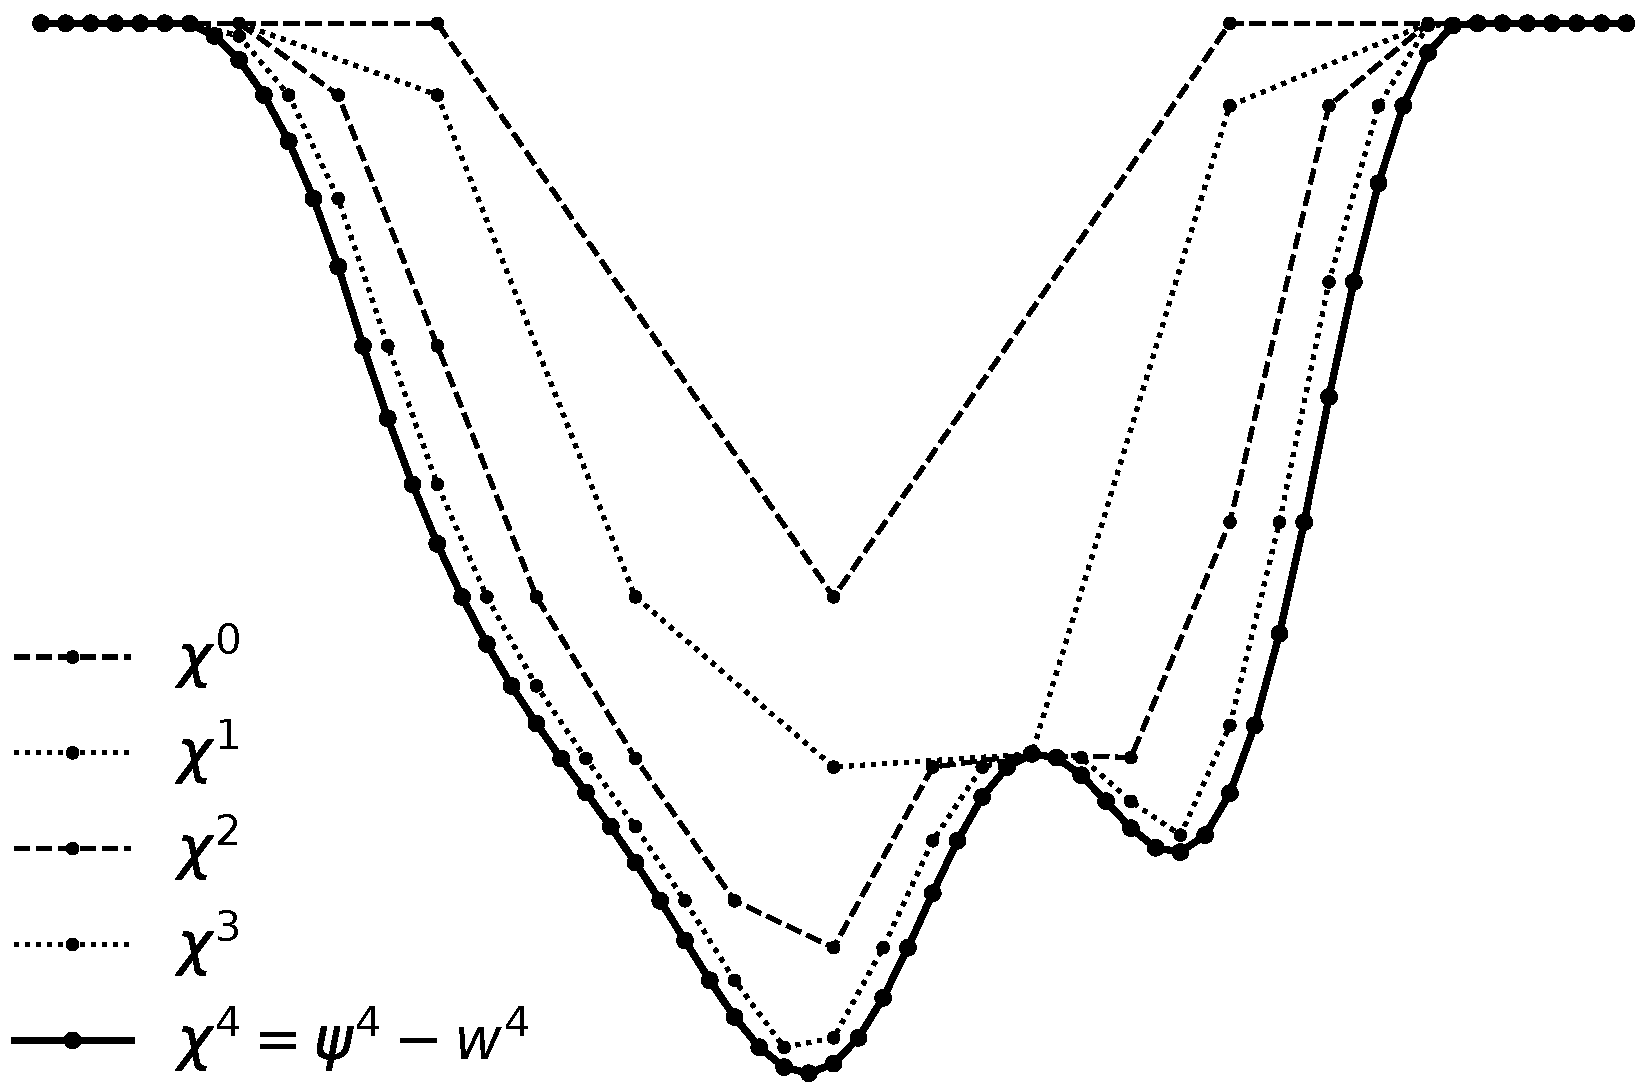
\includegraphics[width=0.65\textwidth]{fixfigs/chiphilevels.pdf}
\caption{The ``below'' level defect constraint (LDC) $\underline{\chi}^J = \underline{\gamma}^J - w^J$ is decomposed using maximum restriction: $\underline{\chi}^{j-1} = \maxR \underline{\chi}^j$.}
\label{fig:chiphilevels}
\end{figure}

Intuitively-speaking, below LDC $\underline{\chi}^j$ generated by maximum restriction $\maxR$, as in \eqref{eq:fe:chilevels}, is the most-negative function from $\mathcal{V}^j$ such that if another element of $\mathcal{V}^j$ is above $\underline{\chi}^j$ then it is also above $\underline{\chi}^{j+1}$ at the finer level.  (Similar comments apply for above LDCs $\overline{\chi}^{j}$.)  In this way, monotone restriction construction of the coarser-level constraints is designed to permit the largest corrections from the coarsest levels \cite{GraeserKornhuber2009}, which promotes V-cycle efficiency.  However, any system satisfying property \eqref{eq:fe:chiordering} will suffice; the particular formula \eqref{eq:fe:chilevels} is not required when generating the LDCs $\underline{\chi}^{j},\overline{\chi}^{j}$.

We then compute the differences between the previous LDCs:
\begin{equation}
\underline{\phi}^j = \underline{\chi}^j - \underline{\chi}^{j-1}, \qquad \overline{\phi}^j = \overline{\chi}^j - \overline{\chi}^{j-1},  \label{eq:fe:philevels}
\end{equation}
using $\underline{\chi}^{-1}=\overline{\chi}^{-1}=0$ to define $\underline{\phi}^0=\underline{\chi}^0$ and $\overline{\phi}^0=\overline{\chi}^0$.  These new nodal functions $\underline{\phi}^{j},\overline{\phi}^{j} \in \tilde{\mathcal{V}}^J$ are also LDCs, and again they bracket zero, $\underline{\phi}^j \le 0 \le \overline{\phi}^j$, but they are not ordered as in \eqref{eq:fe:chiordering}.  However, telescoping sums hold for $j=0,1,\dots,J$:
\begin{equation}
\sum_{i=0}^j \underline{\phi}^i = \underline{\chi}^j, \qquad \sum_{i=0}^j \overline{\phi}^i = \overline{\chi}^j.  \label{eq:fe:telescoping}
\end{equation}
Table \ref{tab:ldcs} should help the reader keep track of these objects.

\begin{table}[H]
\begin{tabular}{llc}
\emph{LDC name}        & \emph{formula} \\ \hline
(finest) upward below & ${\Large \strut} \underline{\chi}^J = \underline{\gamma}^J - w^J$ \\
(finest) upward above & ${\Large \strut} \overline{\chi}^J = \overline{\gamma}^J - w^J$ \\
upward below          & ${\Large \strut} \underline{\chi}^{j} = \maxR \underline{\chi}^{j+1}$ \\
upward above          & ${\Large \strut} \overline{\chi}^{j} = \minR \overline{\chi}^{j+1}$ \\
downward below        & ${\Large \strut} \underline{\phi}^j = \underline{\chi}^j - \underline{\chi}^{j-1}$ \\
downward above        & ${\Large \strut} \overline{\phi}^j = \overline{\chi}^j - \overline{\chi}^{j-1}$ \\
\end{tabular}

\medskip
\caption{Level defect constraints (LDCs) are constructed from the box constraints ($\underline{\gamma}^J,\overline{\gamma}^J$) in problem \eqref{eq:fe:vi}, and a finest level iterate ($w^J \in \cK^J$).}
\label{tab:ldcs}
\end{table}


\section{Multilevel CDs} \label{sec:cdmultilevel}

A multilevel V-cycle solver is defined in the next Section.  For the downward side of the V-cycle we will use the LDCs $\underline{\phi}^j,\overline{\phi}^j$ as constraints, and $\underline{\chi}^j,\overline{\chi}^j$ for the upward side.  The corresponding constraint sets are
\begin{align}
\mathcal{D}^j = \left\{v \in \mathcal{V}^j \,:\, \underline{\phi}^j \le v \le \overline{\phi}^j \text{ and } \, v|_{\partial_D\Omega} = 0\right\}, \label{eq:fe:constraintsets} \\
\mathcal{U}^j = \left\{v \in \mathcal{V}^j \,:\, \underline{\chi}^j \le v \le \overline{\chi}^j \text{ and } \, v|_{\partial_D\Omega} = 0\right\}. \notag
\end{align}
These are the \emph{downward} and \emph{upward defect constraint sets}, respectively, closed and convex subsets of the FE spaces $\mathcal{V}^j$, for $j=0,1,\dots,J$.  Because $\underline{\chi}^j \le \underline{\phi}^j \le 0 \le \overline{\phi}^j \le \overline{\chi}^j$, it follows that $\mathcal{D}^j \subset \mathcal{U}^j$; the upward sets are larger.  Note that the finest-level set $\mathcal{U}^J$ is equivalent to the original constraint set $\mathcal{K}^J$: for all $z^J \in \mathcal{V}^J$,
\begin{equation}
z^J \in \mathcal{U}^J \quad \iff \quad w^J+z^J \in \mathcal{K}^J. \label{eq:fe:finestlevelequivalent}
\end{equation}

Our multilevel strategy is based on constraint decompositions (CDs; Section \ref{sec:cd}) of $\mathcal{U}^J$, or rather incomplete CDs as we now explain.  Each upward set $\mathcal{U}^j$ can be decomposed in an inclusion sense, which becomes a true CD in unilateral cases.  The following Lemma is based on the unilateral CD construction underlying Algorithm 4.7 in \cite{GraeserKornhuber2009}; see also equation (59) in \cite{Tai2003}.  It explains downward admissibility in the V-cycle Algorithm \ref{alg:nmcd} in Section \ref{sec:vcycle}.

\begin{lemma}  \label{lem:downwardadmissibility}  For arbitrary upper and lower obstacles $\underline{\gamma}^J,\overline{\gamma}^J$ satisfying \eqref{eq:fe:boxconstraintrequirements}, and any $j=0,1,\dots,J$,
\begin{equation}
\mathcal{U}^j \supseteq \mathcal{D}^j + \mathcal{D}^{j-1} + \dots + \mathcal{D}^0. \label{eq:fe:downwardsuminclusion}
\end{equation}
In unilateral cases, where either $\underline{\gamma}^J=-\infty$ or $\overline{\gamma}^J=+\infty$, inclusion \eqref{eq:fe:downwardsuminclusion} becomes a full CD \eqref{eq:constraintdecomp}, namely $\mathcal{U}^j=\sum_{i=0}^j \mathcal{D}^i$, over the subspace decomposition $\cV^j=\sum_{i=0}^j \cV^i$.
\end{lemma}

\begin{proof}  Subspace decomposition \eqref{eq:subspacedecomp} holds---see nesting \eqref{eq:fe:nestedspaces}---and definition \eqref{eq:fe:constraintsets} shows $\mathcal{D}^i \subset \cV^i$ and $\mathcal{U}^i \subset \cV^i$.  If $y^i \in \mathcal{D}^i$ for $i=0,\dots,J$ then
\begin{equation}
\underline{\chi}^j = \sum_{i=0}^j \underline{\phi}^i \le \sum_{i=0}^j y^i \le \sum_{i=0}^j \overline{\phi}^i \le \overline{\chi}^j \label{eq:fe:lemmaordering}
\end{equation}
by \eqref{eq:fe:telescoping} and \eqref{eq:fe:constraintsets}, thus \eqref{eq:fe:downwardsuminclusion} holds for any box constraints.

It remains to consider unilateral cases.  Here we can construct decomposition operators and show \eqref{eq:constraintrestrictionsum}.  Suppose $\overline{\gamma}^J=+\infty$, thus $\overline{\chi}^j=+\infty$ and $\overline{\phi}^i = +\infty$ for all levels.  For $v\in \mathcal{V}^j$ and $0\le i \le j$, let $I_{j\to i}^\ominus$ be the operator applying the minimum (monotone) restriction $j-i$ times, mapping into $\mathcal{V}^i$:
\begin{equation}
I_{j\to i}^\ominus v = \minR(\dots(\minR v)\dots)  \label{eq:fe:minimummaps}
\end{equation}
Note that $I_{j\to j}^\ominus v = v$, and set $I_{j\to -1}^\ominus=0$ by definition.  From operators \eqref{eq:fe:minimummaps} we define the nonlinear decomposition operators $\Pi_i:\mathcal{U}^j \to \mathcal{D}^i$:
\begin{equation}
\Pi_i z^j = I_{j\to i}^\ominus(z^j - \underline{\chi}^j) - I_{j\to i-1}^\ominus(z^j - \underline{\chi}^j) + \underline{\phi}^i.  \label{eq:fe:unilateraldecompositionoperator}
\end{equation}
(Compare equation (4.9) in \cite{GraeserKornhuber2009}.)  Property \eqref{eq:fe:monotonerestrictionprops} implies $I_{j\to i}^\ominus(z^j - \underline{\chi}^j) \ge I_{j\to i-1}^\ominus(z^j - \underline{\chi}^j)$, thus $\Pi_i z^j \ge \underline{\phi}^i$, so $\Pi_i z^j \in \mathcal{D}^i$ (in this unilateral case).  On the other hand, the following sum telescopes, leaving only its first term plus the sum in \eqref{eq:fe:telescoping}:
\begin{align*}
\sum_{i=0}^j \Pi_i z^j &= z^j - \underline{\chi}^j + \sum_{i=0}^j \underline{\phi}^i = z^j.
\end{align*}
This shows \eqref{eq:constraintrestrictionsum}, thus that \eqref{eq:fe:downwardsuminclusion} is equality, a true CD \eqref{eq:constraintdecomp}.

The case where $\underline{\gamma}^J=-\infty$ is similar.
\end{proof}

It is tempting to try to turn \eqref{eq:fe:downwardsuminclusion} into a full CD for arbitrary box constraints by using decomposition maps like $\Pi_i$.  Specifically, one might split $z^j = \min\{z^j,0\} + \max\{z^j,0\}$ and apply unilateral formulas like \eqref{eq:fe:unilateraldecompositionoperator} to $\min\{z^j,0\}$ and $\max\{z^j,0\}$ separately, with $\Pi_i$ applied to $\min\{z^j,0\}$ and a straightforward variant operator to $\max\{z^j,0\}$.  In fact, the lower bound $\Pi_i (\min\{z^j,0\}) \ge \underline{\phi}^i$ holds, as shown in the above proof.  However, the following Example shows why $\Pi_i(\min\{z^j,0\})$ may have an arbitrarily large maximum, and thus exceed any finite upper LDC $\overline{\phi}^i$, so unfortunately $\Pi_i$ does not map even non-positive functions to $\mathcal{D}^i$ in the presence of a finite upper LDC.  While the proposed splitting strategy does not work, without redefinition of a formula which is adequate in the unilateral case, the existence of an entirely-different strategy for showing a full CD is also not excluded.

\begin{example}  \label{ex:notfullcd}
Let $a\ge 0$ be an arbitrary positive number.  Consider a 2-level hierarchy ($J=1$), and suppose the lower defect constraint is the constant function $\underline{\chi}^1=-a$.  Recalling Table \ref{tab:ldcs}, note $\underline{\chi}^0=\maxR \underline{\chi}^1=-a$ also, so $\underline{\phi}^1=0$ and $\underline{\phi}^0=-a$.  Suppose $z^1$ is a ``sawtooth'' function which takes on value $-a$ on the coarse nodes and value $0$ on the other fine-level nodes.  Then $\overline{\chi}^1 \ge 0 \ge z^1\ge \underline{\chi}^1$, for any valid $\overline{\chi}^1$, so $z^j \in \mathcal{U}^1$.  However, $I_{1\to 0}^\ominus(z^1 - \underline{\chi}^1) = \minR(z^1 - \underline{\chi}^1) = 0$ identically.  From \eqref{eq:fe:unilateraldecompositionoperator}, $\Pi_1 z^1$ simplifies to $\Pi_1 z^1 = z^1 - \underline{\chi}^1$.  But then $\Pi_1 z^1$ attains a maximum $a\ge 0$.  This maximum can be chosen to exceed any upper defect obstacle $\overline{\phi}^1$.  Thus, for general $w^1 \in \mathcal{U}^1$ and general LDCs, $\Pi_1$ does not map $\min\{w^1,0\}$ into $\mathcal{D}^1$.
\end{example}

Each upward defect constraint set $\mathcal{U}^j$ can also be be decomposed down to an arbitrary level $k$ where an upward set $\mathcal{U}^k$ is used as the coarsest set.  The next Lemma, similar to Lemma \ref{lem:downwardadmissibility} but not following from it, explains upward admissibility in V-cycle Algorithm \ref{alg:nmcd}.

\begin{lemma}  \label{lem:upwardadmissibility}  For any $j=0,1,\dots,J$ and $0\le k\le j$,
\begin{equation}
\mathcal{U}^j \supseteq \mathcal{D}^j + \mathcal{D}^{j-1} + \dots + \mathcal{D}^{k+1} + \mathcal{U}^k \label{eq:fe:upwardsuminclusion}
\end{equation}
In unilateral cases, where either $\underline{\gamma}^J=-\infty$ or $\overline{\gamma}^J=+\infty$, inclusion \eqref{eq:fe:upwardsuminclusion} is a full CD \eqref{eq:constraintdecomp}. \end{lemma}

\begin{proof}  Definition \eqref{eq:fe:philevels} shows that $\underline{\chi}^j = \underline{\phi}^j + \dots + \underline{\phi}^{k+1} + \underline{\chi}^k$ and $\overline{\chi}^j = \overline{\phi}^j + \dots + \overline{\phi}^{k+1} + \overline{\chi}^k$.  (These facts replace \eqref{eq:fe:telescoping}.)  If $y^i \in \mathcal{D}^i$ for $i=k+1,\dots,j$ and $z^k \in \mathcal{U}^k$ then it is easy to show, as in \eqref{eq:fe:lemmaordering}, that $\underline{\chi}^j \le y^j + \dots + y^{k+1} + z^k \le \overline{\chi}^j$, thus \eqref{eq:fe:upwardsuminclusion} holds.

In unilateral cases we follow the proof of Lemma \ref{lem:downwardadmissibility}.  Definition \eqref{eq:fe:minimummaps} is unchanged.  We use \eqref{eq:fe:unilateraldecompositionoperator} unchanged for $i=k+1,\dots,j$, but modify it in the $i=k$ case: $\Pi_k z^j = I_{j\to k}^\ominus(z^j - \underline{\chi}^j) + \underline{\chi}^k$.  The remainder of the proof goes through as for Lemma \ref{lem:downwardadmissibility}.
\end{proof}

In summary, inclusions \eqref{eq:fe:downwardsuminclusion} and \eqref{eq:fe:upwardsuminclusion} suffice to show the admissibility of all iterates and corrections in V-cycle Algorithm \ref{alg:nmcd}.  However, a convergence analysis following \cite{Tai2003} or \cite{GraeserKornhuber2009}, somehow extending their arguments to VIs \eqref{eq:vi} which are not of minimization type, or to box constraints, would seem to require full CDs, and perhaps new ideas.


\section{Nonlinear multilevel constraint decomposition (NMCD) V-cycle} \label{sec:vcycle}

The \emph{nonlinear multilevel constraint decomposition} (NMCD) V-cycle algorithm in this section uses CDs \eqref{eq:fe:downwardsumcd} and \eqref{eq:fe:upwardsumcd}.  It does smoothing in $\mathcal{D}^j$ for the downward direction, and $\mathcal{U}^j$ for the upward direction, respectively, in the V-cycle.  The algorithm generalizes the multilevel CD schemes of Tai \cite{Tai2003} and Gr\"aser \& Kornhuber \cite[Algorithm 4.7]{GraeserKornhuber2009} by following a nonlinear \emph{full approximation scheme} (FAS) approach \cite{BrandtLivne2011}.  We coarsen the solution iterate itself, using injection, in constrast to classical linear multigrid wherein only the residual is coarsened.

The finest-level iterate $w^J \in \mathcal{K}^J$ will be corrected by perturbations from each coarser subspace $\mathcal{V}^j$,\footnote{By nesting \eqref{eq:fe:nestedspaces} these corrections also live in the fine-level subspace $\mathcal{V}^J$.  Later we will use prolongation $P$ to indicate where a change in computer representation would be needed.} but the corrected iterate needs to be admissible.  In detail, suppose $y^J \in \mathcal{D}^J, y^{J-1} \in \mathcal{D}^{J-1}, \dots, y^{j+1} \in \mathcal{D}^{j+1}$ are already-computed corrections during the downward part of the V-cycle (Figure \ref{fig:nmcdvcycle}).  By \eqref{eq:fe:downwardsumcd} the corrected iterate at this point is admissible, namely $y^J + \dots + y^{j+1} \in \mathcal{U}^J$, equivalently $w^J + y^J + \dots + y^{j+1} \in \mathcal{K}^J$.  Smoothing then happens at the next-coarser level $j$, i.e.~we incompletely-solve VI problem \eqref{eq:fe:downvi} below.  At the bottom the coarsest-level VI is then (accurately) solved, to generate the full downslash correction $y^J + \dots + y^1 + z^0 \in \mathcal{U}^J$.  Starting upward, however, we can use $y^1+ z^0 \in \mathcal{U}^1$ as an initial iterate on level $j=1$, and then smooth by incompletely-solving VI problem \eqref{eq:fe:upvi} (below) in $\mathcal{U}^1$, yielding admissible total correction $y^J + \dots + y^2 + z^1 \in \mathcal{U}^J$ using \eqref{eq:fe:upwardsumcd}.  Continuing in this ``telescoping'' way, up-smoothing in the constraint sets $\mathcal{U}^j$ from initial iterate $y^j+z^{j-1}$, eventually generates $z^J\in \mathcal{U}^J$ as the full V-cycle correction, yielding the new iterate $w^J + z^J \in \mathcal{K}^J$.

\begin{figure}[ht]
\begin{center}
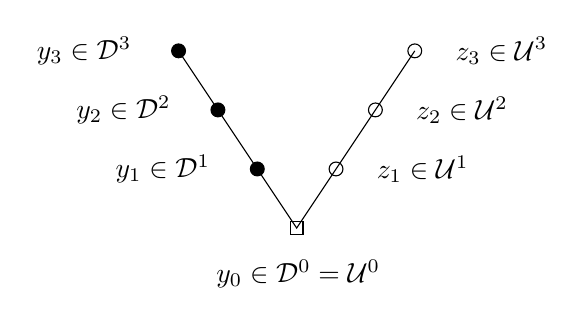
\begin{tikzpicture}[scale=1.0]
  \pgfmathsetmacro\hstep{0.5}
  \pgfmathsetmacro\vstep{0.75}
  \pgfmathsetmacro\ceps{0.08}   % size of square for coarse grid

% V-cycle with MCD down-obstacle and up-obstacle annotations
  \draw[black,thin] (-\hstep,3*\vstep) -- (0.0,2*\vstep) -- (\hstep,\vstep) --  (2*\hstep,0.0)
                    -- (3*\hstep,\vstep) -- (4*\hstep,2*\vstep) -- (5*\hstep,3*\vstep);
  \filldraw (-\hstep,3*\vstep) node[xshift=-12mm] {$y_3 \in \mathcal{D}^3$} circle (2.5pt);
  \filldraw (0.0,2*\vstep) node[xshift=-12mm] {$y_2 \in \mathcal{D}^2$} circle (2.5pt);
  \filldraw (\hstep,\vstep) node[xshift=-12mm] {$y_1 \in \mathcal{D}^1$} circle (2.5pt);
  \draw     (2*\hstep-\ceps,-\ceps) node[xshift=1mm,yshift=-5mm] {$y_0 \in \mathcal{D}^0 = \mathcal{U}^0$} rectangle (2*\hstep+\ceps,+\ceps);
  \draw     (3*\hstep,\vstep) node[xshift=11mm] {$z_1 \in \mathcal{U}^1$} circle (2.5pt);
  \draw     (4*\hstep,2*\vstep) node[xshift=11mm] {$z_2 \in \mathcal{U}^2$} circle (2.5pt);
  \draw     (5*\hstep,3*\vstep) node[xshift=11mm] {$z_3 \in \mathcal{U}^3$} circle (2.5pt);
\end{tikzpicture}

\end{center}
\caption{An NMCD V-cycle computes downward corrections $y_j \in \mathcal{D}^j$ and upward corrections $z_j\in\mathcal{U}^j$.  The latter live in larger constraint subsets.}
\label{fig:nmcdvcycle}
\end{figure}

A key idea, implicit in the above paragraph, is that the up-smoothing stages solve less-restricted VI problems than down-smoothing stages.  Intuitively-speaking, downward one does not know what the coarse corrections will be, so they must be in such small sets ($\mathcal{D}^j$) that their sum is admissible once we return to the current level.  However, going upward smoothing can occur in the larger admissible-sum sets ($\mathcal{U}^j$; see \eqref{eq:fe:constraintdecomp}) because there are no forthcoming coarser corrections which could violate admissibility.

To justify the NMCD algorithm---see Algorithm \ref{alg:nmcd} below---we must state the problems solved at each mesh level.\footnote{Smoothers/solvers for these problems are proposed in Section \ref{sec:smoothers}.}  As in classical FAS multigrid for nonlinear PDEs \cite{BrandtLivne2011,Bruneetal2015,Trottenbergetal2001}, both the solution approximation and the residual must be coarsened, along with creating a source functional.  Recall that Table \ref{tab:transfers} summarizes the needed transfer operators.

Let $j$ denote the mesh level of the coarsened problem.  We assume a (re-)discretized nonlinear operator $f^j$, with output in $(\cV^j)'$, an FE discretization of $f$ in \eqref{eq:boxdirichletvi}, using quadrature and etc., presumably by the same scheme which generated $f^J$ in \eqref{eq:fe:vi}.

The formulas are as follows.  Finest-level problem \eqref{eq:fe:vi} is defined by the discretized operator $f^J$ and the original source functional $\ell^J$.  A finest-level, admissible iterate $w^J \approx u^J$, $w^J \in \mathcal{K}^J$, has already\footnote{Conceptually-speaking, at least.  In practice one generates LDCs $\underline{\chi}^j,\overline{\chi}^j,\underline{\phi}^j,\overline{\phi}^j$ during the descent stage; see Algorithm \ref{alg:nmcd}.  Observe that the LDCs depend neither on coarsened iterates $g^j$ nor corrections $y^j,z^j$.} been used to general the LDCs and constraint sets $\mathcal{D}^j,\mathcal{U}^j$ at each level (Section \ref{sec:femultilevel}).  As we descend in the V-cycle, we recursively define $j$th-level iterates
\begin{equation}
g^j = \begin{cases} w^J, & j=J \\
                    \iR(g^{j+1} + y^{j+1}), & j < J.
      \end{cases}  \label{eq:fe:defineg}
\end{equation}
These are the iterates \emph{before} smoothing and/or correction has been applied at level $j$.  (The problem solved by $y^{j+1}$ is stated momentarily.)  From $g^j$ we define $\ell^j \in (\cV^j)'$:
\begin{equation}
\ell^j = \begin{cases} \ell^J, & j=J \\
                       f^j(g^j) + R\left(\ell^{j+1}-f^{j+1}(g^{j+1}+y^{j+1})\right), & j<J. \end{cases} \label{eq:fe:levelsource}
\end{equation}
Observe that injection $\iR$ coarsens the iterates $g^j$---injection is commonly used in classical FAS \cite[section 5.3]{Trottenbergetal2001}---while canonical restriction $R$ coarsens the source functionals.

On descent, $j=J,J-1,\dots,1$, we solve the following VI for $y^j \in \mathcal{D}^j$:
\begin{equation}
\ip{f^j(g^j + y^j)}{v-y^j} \ge \ip{\ell^j}{v-y^j} \qquad \text{for all } v\in \mathcal{D}^j, \label{eq:fe:downvi}
\end{equation}
for which the initial iterate is
\begin{equation}
(y^j)^{(0)}=0.  \label{eq:fe:downwardinitial}
\end{equation}
(Zero is admissible; see the comment after \eqref{eq:fe:philevels}.)  On ascent, $j=0,1,\dots,J$, the same VI is solved, but in a larger admissible set.  We find $z^j \in \mathcal{U}^j$ so that
\begin{equation}
\ip{f^j(g^j + z^j)}{v-z^j} \ge \ip{\ell^j}{v-z^j} \qquad \text{for all } v\in \mathcal{U}^j. \label{eq:fe:upvi}
\end{equation}
The nontrivial initial iterate for this problem is found by prolonging the coarser-level correction $z^{j-1}$, and using it to correct the current (down-smoothed) iterate on the level:\footnote{Prolongation $P$ is used in \eqref{eq:fe:upwardinitial} to reflect the change in mesh/FE representation, from $\mathcal{T}^{j-1}$ to $\mathcal{T}^{j}$.}
\begin{equation}
(z^j)^{(0)} = y^j + P z^{j-1}.  \label{eq:fe:upwardinitial}
\end{equation}
For the $j=0$ coarsest level, $(z^0)^{(0)}=0$.  Initial iterate \eqref{eq:fe:upwardinitial} is admissible since $\mathcal{U}^j = \mathcal{D}^j + \mathcal{U}^{j-1}$; see \eqref{eq:fe:constraintdecomp} or \eqref{eq:fe:upwardsumcd}.

If we were to inject the original bi-obstacles from \eqref{eq:fe:fineconstraintset} downward to coarser meshes, i.e.~$\underline{\gamma}^j = \iR \underline{\gamma}^{j+1}$ and $\overline{\gamma}^j = \iR \overline{\gamma}^{j+1}$, then, because injection preserves inequalities, and because $y^{j+1} \in \mathcal{D}^{j+1}$, it would follow from \eqref{eq:fe:defineg} that $\underline{\gamma}^j \le g^j \le \overline{\gamma}^j$, just like $\underline{\gamma}^J \le w^J \le \overline{\gamma}^J$ for the finest-level iterate.  In this narrow sense $g^j$ is admissible with respect to the original (finest-level) box constraints.  (In fact, while $g^j \in \cV^j \subset \cV^J$ certainly holds, generally $g^j \notin \cK^J$.)  However, following \cite{GraeserKornhuber2009}, our use of defect constraints (Table \ref{tab:ldcs}) avoids the need to generate functions $\underline{\gamma}^j$ and $\overline{\gamma}^j$, and it yields a final, finest-level iterate $g^J+z^J \in \cK^J$ which is genuinely admissible for problem \eqref{eq:fe:vi}.

Regarding formula \eqref{eq:fe:levelsource}, the source function $\ell^j$ is determined by a classical FAS-type formula.  (Compare equation (8.5b) in \cite{BrandtLivne2011} or equation (5.3.14) in \cite{Trottenbergetal2001}.)  It has the following explanation, mimicking the PDE story from textbooks, which simultaneously justifies \eqref{eq:fe:levelsource} and VI problems \eqref{eq:fe:downvi} and \eqref{eq:fe:upvi}.  First, the $j+1$ level problem \eqref{eq:fe:downvi} is not solved exactly by the finer-level correction $y^{j+1}$; the down-smoother was only approximate.  Conceptually, we seek a further correction $y$ on the $j+1$ level so that
\begin{equation}
\ip{f^{j+1}(g^{j+1}+y^{j+1}+y)}{v-y^{j+1}-y} \ge \ip{\ell^{j+1}}{v-y^{j+1}-y}, \, \forall v\in \mathcal{D}^j \quad \text{\emph{(notional)}} \label{eq:fe:downvinotional}
\end{equation}
holds exactly.  However, $y$ will actually be approximated from a problem on the next-coarser level.  This $j$th-level problem comes from modifying notional VI \eqref{eq:fe:downvinotional} in 4 steps:
\begin{enumerate}
\item subtract the computable quantity $f^{j+1}(g^{j+1}+y^{j+1}) \in (\mathcal{V}^{j+1})'$ from both sides,
\item replace the residual $\ell^{j+1}-f^{j+1}(g^{j+1}+y^{j+1})$, now on the right, by its restriction,
\item replace $g^{j+1}+y^{j+1}$, where it appears on the left, by its restriction,
\item and, where it appears on the left, replace $f^{j+1}$ by its coarser rediscretization $f^j$.
\end{enumerate}
Steps \emph{(ii)}--\emph{(iv)} are justified, as for PDEs \cite[subsection 5.3.4, for example]{Trottenbergetal2001}, because the residual and the error should be smooth as a result of the progress made by the $j+1$ level down-smoother.  These steps now yield a problem for the $j$th-level correction $y^j \in \mathcal{D}^j$:
\begin{align}
&\ip{f^j\left(\iR(g^{j+1}+y^{j+1})+y^j\right)}{v-y^j} - \ip{f^j\left(\iR(g^{j+1}+y^{j+1})\right)}{v-y^j} \label{eq:fe:downvicluttered} \\
&\qquad \ge \ip{R\left(\ell^{j+1}-f^{j+1}(g^{j+1}+y^{j+1})\right)}{v-y^j} \notag
\end{align}
This is the same as VI problem \eqref{eq:fe:downvi}, but in cluttered form; application of definitions \eqref{eq:fe:defineg} and \eqref{eq:fe:levelsource} yields \eqref{eq:fe:downvi}.  The explanation for VI \eqref{eq:fe:upvi} is essentially identical.

We will regard the smoothers for VI problems \eqref{eq:fe:downvi} and \eqref{eq:fe:upvi} as approximate, in-place procedures, acting on the corrections $y^j$ and $z^j$, respectively.  Also, as is standard in multigrid, at the coarsest $j=0$ level we suppose that problem \eqref{eq:fe:upvi} is solved quite accurately.  However, this coarsest-level solver may be the same as the other smoothers, perhaps with a stronger tolerance.

These ideas come together in Algorithm \ref{alg:nmcd}, below.  The \pr{nmcd-vcycle} procedure acts in-place on $w^J$, but it leaves its other inputs unchanged.

\begin{pseudofloat}[ht]
\begin{pseudo} \label{ps:nmcd-vcycle}
\pr{nmcd-vcycle}(\ell^J,\underline{\gamma}^J,\overline{\gamma}^J;w^J)\text{:} \\+
    $\underline{\chi}^J = \underline{\gamma}^J - w^J {\large \strut}$ \\
    $\overline{\chi}^J = \overline{\gamma}^J - w^J {\large \strut}$ \\
    $g^J = w^J$ \\
    for $j=J$ downto $j=1$ \\+
      $\underline{\chi}^{j-1} = \maxR \underline{\chi}^j {\large \strut}$ \\
      $\overline{\chi}^{j-1} = \minR \overline{\chi}^j {\large \strut}$ \\
      $\underline{\phi}^j = \underline{\chi}^j - P\underline{\chi}^{j-1} {\large \strut}$ \\
      $\overline{\phi}^j = \overline{\chi}^j - P\overline{\chi}^{j-1} {\large \strut}$ \\
      $y^j = 0$ \\
      $\text{\pr{smooth}}^{\text{\id{down}}}(\ell^j,\underline{\phi}^j,\overline{\phi}^j,g^j;y^j)$  \ct{smoothing of \eqref{eq:fe:downvi} in $\mathcal{D}^j$}\\
      $g^{j-1} = \iR(g^j + y^j)$ \\
      $\ell^{j-1} = f^{j-1}(g^{j-1}) + R \left(\ell^j - f^j(g^j+y^j)\right)$ \\-
    $z^0 = 0$ \\
    $\text{\pr{solve}}(\ell^0,\underline{\chi}^0,\overline{\chi}^0,g^0;z^0)$ \hspace{1.0cm} \ct{solving of \eqref{eq:fe:upvi} in $\mathcal{U}^0$} \\
    for $j=1$ to $j=J$ \\+
      $z^j = y^{j} + P z^{j-1}$ \\
      $\text{\pr{smooth}}^{\text{\id{up}}}(\ell^j,\underline{\chi}^j,\overline{\chi}^j,g^j;z^j)$  \ct{smoothing of \eqref{eq:fe:upvi} in $\mathcal{U}^j$} \\-
    $w^J \gets w^J+z^J$
\end{pseudo}
\caption{Nonlinear multilevel constraint decomposition V-cycle as an iterative solver for FE VI problem \eqref{eq:fe:vi}.  $f^j$ denotes an FE discretization of $f$ in problem \eqref{eq:boxdirichletvi}.}
\label{alg:nmcd}
\end{pseudofloat}

Regarding its efficiency, to begin we consider storage.  One application of \pr{nmcd-vcycle}, assuming all box constraints are nontrivial, storage must be allocated for the seven vectors $\underline{\chi}^j$, $\overline{\chi}^j$, $\underline{\phi}^j$, $\overline{\phi}^j$, $g^j$, $\ell^j$, and $y^j$ on each level.  (Note $z^J$ can use the same storage as $y^j$.)  On the finest level one must also store $\underline{\gamma}^J$ and $\overline{\gamma}^J$, but note $g^J=w^J$ are the same.  On the coarsest level there are only five vectors to store.  Therefore, using estimates for 2D refinement plus a standard geometric series argument \cite{Trottenbergetal2001}, the total storage of a deep $V$-cycle, excluding the implementations of smoothers and the coarse-level solver, is about
\begin{equation}
9 m_J + 7 m_{J-1} + \dots + 7 m_1 + 5 m_0 \approx \left(9 + 7 \sum_{k=1}^\infty \frac{1}{4^k}\right) m_J \approx 11 m_J
\end{equation}
real numbers.  For comparison, a single-level method needs at least $4 m_J$ storage for the vectors $\underline{\gamma}^J,\overline{\gamma}^J,\ell^J,w^J$.  If some of the obstacles are trivial, for instance if $\overline{\gamma}^J=+\infty$ in a unilateral obstacle problem, storage is correspondingly reduced at all levels.

\pr{nmcd-vcycle} assumes certain semantics for the smoothers \pr{smooth} and the coarsest-level solver \pr{solve}.  These solvers do in-place modifications of their final arguments, without modifying their first four arguments.  $\pr{smooth}^{\id{down}}$ and $\pr{smooth}^{\id{up}}$ are in-exact solvers of VIs \eqref{eq:fe:downvi} and \eqref{eq:fe:upvi}, respectively, iterated \id{down} and \id{up} times.  Further implementation details are addressed in Section \ref{sec:smoothers}.

Repeated application of \pr{nmcd-vcycle} to solve VI \eqref{eq:fe:vi} will not reduce the finest-level residual $f^J(w^J) - \ell^J$ to zero everywhere, and we need to identify the vector quantity whose norm must be controlled by a tolerance.  Recalling the comments following mixed complementarity problem \eqref{eq:fe:mcp}, and denoting the hat function at node $x_p \in \mathcal{T}^J$ by $\psi_p$, for $w^J \in \mathcal{K}^J$ we define the following vector in $\RR^{m_J}$ as the finest-level \emph{nodal complementarity residual} which is defined as follows in the four cases (inactive, lower active, upper active, boundary):\footnote{Formally-speaking, $\hat r:\mathcal{V}^J \to \RR^{m_J}$ is simply a computable nonlinear map derived from $f^J$ and the vectors $\ell^J$, $\underline{\gamma}^J$, and $\overline{\gamma}^J$.  It is an important part of the implementation.}
\begin{equation}
\hat r(w^J)_p = \begin{cases}
    \ip{f^J(w^J)-\ell^J}{\psi_p}, & \underline{\gamma}^J(x_p) < w^J(x_p) < \overline{\gamma}^J(x_p), \\
    \min\{\ip{f^J(w^J)-\ell^J}{\psi_p},0\}, & w^J(x_p) = \underline{\gamma}^J(x_p), \\
    \max\{\ip{f^J(w^J)-\ell^J}{\psi_p},0\}, & w^J(x_p) = \overline{\gamma}^J(x_p), \\
    0, & x_p \in \partial_D\Omega. \end{cases} \label{eq:cpresidual}
\end{equation}
The point is that $\hat r(w^J)\in \RR^{m_J}$ is nonzero if there are nodes where MCP \eqref{eq:fe:mcp} is violated, either because the pointwise classical residual $\ip{f^J(w^J)-\ell^J}{\psi_p}$ remains nonzero where the constraints are inactive, or because it has the wrong sign on an actively-constrained degree of freedom.

A solver for \eqref{eq:fe:vi} using repeated applications of \pr{nmcd-vcycle} would start with an initial iterate $(w^J)^{(0)}$, do V-cycles, and stop once the finest-level nodal residual $\hat r(w^J)$ was sufficiently small.  For example, using tolerances \id{atol}$>0$ and \id{rtol}$>0$ the stopping criterion might be
\begin{equation}
\|\hat r(w^J)\| < \id{atol} \qquad \text{or} \qquad \frac{\|\hat r(w^J)\|}{\|\hat r((w^J)^{(0)})\|} < \id{rtol},
\end{equation}
for some norm $\|\cdot\|$ on $\RR^{m_J}$.  A step tolerance could also be used, measuring the difference between successive iterates.


\section{Smoother implementations} \label{sec:smoothers}

FIXME  Recall that a $j$th-level hat function based at node $x_p^j$ is denoted $\psi_p^j$, for an iterate $g^j$ and an admissible correction $y^j \in \mathcal{D}^j$ we define the \emph{downward nodal residual} as
\begin{equation}
(\hat r_{\text{down}}(y^j))_p = \begin{cases} \ip{f^j(g^j+y^j)-\ell^j}{\psi_p^j}, & y^j(x_p^j) > \phi^j(x_p^j), \\
                                  \min\{\ip{f^j(g^j+y^j)-\ell^j}{\psi_p^j},0\}, & y^j(x_p^j) = \phi^j(x_p^j). \end{cases} \label{eq:dncpresidual}
\end{equation}
The \emph{upward nodal residual} $\hat r_{\text{up}}(z^j)$ for $z^j \in \mathcal{U}^j$ is similarly defined using $\chi^j$.

FIXME stopping criteria for smoother


\section{Results and discussion} \label{sec:results}

FIXME show results for 2D Firedrake implementation of NMCD for $p$-Laplacian obstacle problem (Example \ref{ex:plaplacian}), advection-diffusion obstacle problem (Example \ref{ex:advectiondiffusion}), and porous-media obstacle problem (Example \ref{ex:porous})

FIXME observe that up-smoothing is more efficient; this observation seems to be new; compare the comments on V(1,0) and V(1,1) cycles in \cite{GraeserKornhuber2009,Tai2003}

FIXME constrast the implemented examples in \cite{GraeserKornhuber2009,Tai2003} in which $f$ is linear

FIXME in Appendix we show how NMCD reduces to FAS if the obstacle is removed and to MCD if $f$ is assumed to be linear

% A BRIDGE TOO FAR:  \section{Results for a nonlocal variational inequality}


\bibliography{mcd2}
\bibliographystyle{siam}


\appendix
\section{Reductions of NMCD to familiar multilevel algorithms}

Algorithm \ref{alg:nmcd} in the main text, \pr{nmcd-vcycle}, generalizes two better-known multilevel algorithms.  First we show that it reduces to the FAS multigrid V-cycle for nonlinear PDEs (which itself generalizes the standard linear multigrid V-cycle \cite{Trottenbergetal2001}).  Second we reduce NMCD to an existing MCD V-cycle for unilateral linear variational inequalities \cite{GraeserKornhuber2009}.  This Appendix helps readers understand Algorithm \ref{alg:nmcd} by separating those assumptions which relate to nonlinear and FAS aspects from the nontrivial modifications of standard multigrid which are caused by inequality constraints.  The later arise even when $f$ in \eqref{eq:vi} is a linear operator.

To derive the classical FAS multigrid V-cycle from Algorithm \ref{alg:nmcd}, we remove the inequality constraints from VI problem \eqref{eq:fe:vi} and then simplify the pseudocode accordingly.  To do this we suppose that the finest-level obstacles $\underline{\gamma}^J$ and $\overline{\gamma}^J$ are very negative and positive, respectively, with magnitude exceeding $u^J$ or any prospective iterate $w^J$.  Finest-level problem \eqref{eq:fe:vi} is then unconstrained except for its Dirichlet boundary conditions.  Let $\mathcal{V}_0^J \subset \mathcal{V}^J$ denote the space with zero values on $\partial_D\Omega$.  By replacing ``$v-u^J$'' with an arbitrary $v \in \mathcal{V}_0^J$ we have the finest-level, weak form problem
\begin{equation}
\ip{f^J(u^J)}{v} = \ip{\ell^J}{v} \qquad \text{for all } v\in \mathcal{V}_0^J \label{eq:app:fas:pde}
\end{equation}
corresponding to the strong-form PDE $f(u)=\ell$.

Furthermore, the downward $\mathcal{D}^j$ and upward $\mathcal{U}^j$ constraint sets can be arbitrarily enlarged so that the coarser-level corrections $y^j$ and $z^j$ in Algorithm \ref{alg:nmcd} are also never constrained.  Formally-speaking we might do this, still satisfying the LDC ordering property \eqref{eq:fe:chiordering}, by choosing LDCs with all gaps being large so that $\underline{\chi}^j \ll 0 \ll \overline{\chi}^j$ and also $\underline{\phi}^j = \underline{\chi}^j - \underline{\chi}^{j-1} \ll 0 \ll \overline{\phi}^j = \overline{\chi}^j - \overline{\chi}^{j-1}$.\footnote{As noted after \eqref{eq:fe:chiordering}, the application of monotone restriction operators $\maxR,\minR$ is not required to generate LDCs $\underline{\chi}^j$ and $\overline{\chi}^j$ satisfying the ordering property.}

Now the correction VIs \eqref{eq:fe:downvi} and \eqref{eq:fe:upvi} are also unconstrained, and lines 2--3 and 6--9 can be removed from Algorithm \ref{alg:nmcd}.  Also, because the downward corrections $y^j$ are no longer separately constrained, we may simply refer to the corrected solution $w^j=g^j+y^j$ instead of $g^j$ and $y^j$ separately.  Then the smoothers and the coarsest-level solver can be regarded as in-place modifications of $w^j$.  Now noting $g^{j-1}=\iR w^j$ in line 12, after down-smoothing, the coarsened source functional can be rewritten using notation $w^{j-1}=\iR w^j$:
\begin{equation}
\ell^{j-1} = f^{j-1}\left(w^{j-1}\right) + R\left(\ell^j-f^j(w^j)\right). \label{eq:app:fas:levelsource}
\end{equation}
(Compare line 13 of Algorithm \ref{alg:nmcd}.)

At the completion of down-smoothing the solution iterate on the $j$th level is $w^j=g^j+y^j$.  Now we must be careful that going upward only the coarse correction, and not the coarse solution, gets prolonged.\footnote{Compare Remark 5.3.9 in \cite{Trottenbergetal2001}, a warning to novices.}  The coarser-level iterate is $w^{j-1} = g^{j-1}+z^{j-1}$ after up-smoothing on the $j-1$ level.  From Algorithm \ref{alg:nmcd} the initial value of the correction $z^j$, before smoothing, is $z^j = y^j + P z^{j-1}$.  These facts imply that the $j$th-level iterate before up-smoothing must be set to
    $$w^j \gets w^j + Pz^j = (g^j+y^j)+P(w^{j-1} - g^{j-1}) = w^j + P(w^{j-1} - \iR w^j).$$
This is a standard FAS statement.  In fact, with the given modifications, we have the much-simplified pseudocode in Algorithm \ref{alg:fas}.  This FAS V-cycle algorithm appears in various places, for example Algorithm 14 of \cite{Bruneetal2015} or in section 5.3.4 of \cite{Trottenbergetal2001}.

\begin{pseudofloat}[ht]
\begin{pseudo} \label{ps:fas-vcycle}
\pr{fas-vcycle}(\ell^J; w^J)\text{:} \\+
    for $j=J$ downto $j=1$ \\+
      $\text{\pr{smooth}}^{\text{\id{down}}}(\ell^j;w^j)$ \\
      $w^{j-1} = \iR w^j$ \\
      $\ell^{j-1} = f^{j-1}(w^{j-1}) + R \left(\ell^j - f^j(w^j)\right)$ \\-
    $\text{\pr{solve}}(\ell^0;w^0)$ \\
    for $j=1$ to $j=J$ \\+
      $w^j \gets w^j + P (w^{j-1} - \iR w^j)$ \\
      $\text{\pr{smooth}}^{\text{\id{up}}}(\ell^j;w^j)$ \\-
\end{pseudo}
\caption{An FAS V-cycle results from removing the inequality constraints from \pr{nmcd-vcycle}, and simplifying accordingly.}
\label{alg:fas}
\end{pseudofloat}

FIXME by assuming $f$ is linear, reduce to Algorithm 4.7 in \cite{GraeserKornhuber2009} but with $\text{V}(\nu_1,\nu_2)$ cycles

\end{document}

